\documentclass[conference]{IEEEtran}
\IEEEoverridecommandlockouts
% The preceding line is only needed to identify funding in the first footnote. If that is unneeded, please comment it out.
\usepackage{cite}
\usepackage{amsmath,amssymb,amsfonts}
\usepackage{algorithmic}
\usepackage{graphicx}
\usepackage{textcomp}
\usepackage{xcolor}
\usepackage{float}
\usepackage{cleveref}
\usepackage{epstopdf}


\usepackage[T1]{fontenc}
\usepackage[utf8]{inputenc}
\def\BibTeX{{\rm B\kern-.05em{\sc i\kern-.025em b}\kern-.08em
    T\kern-.1667em\lower.7ex\hbox{E}\kern-.125emX}}


\DeclareMathOperator{\atantwo}{atan2}



\begin{document}

\title{Aarhus University MSc Course Project  \\ Control of Mobile Robots}

\author{\IEEEauthorblockN{S. L. Skovgaard and D. Tøttrup}
\IEEEauthorblockA{\textit{dept. of Engineering (of Aff.)} \\
\textit{Aarhus Unitversity (of Aff.)}\\
Aarhus, Denmark \\
201401682@post.au.dk \\
201509520@post.au.dk}}

\maketitle

\begin{abstract}

This document is the final project in the course Control of Mobile Robots. This final project focus on designing and implementing a PID-controller, that is able to control a Parrot Bebop 2 UAV in real world lab environment and investigating what influence the different controller parameters have. To accomplish this it is necessary to transform linear velocity and angular rates in inertial coordinates into the UAV's body frame. The project consist of two tasks. The first task involves the UAV hovering in a specific point 1 meter above the ground while being exposed to disturbances. The second task involve the UAV flying in a square shape trajectory by visiting the way-points (0,0,1), (2,0,1), (2,2,1) and (0,2,1) with an arbitrary yaw angle. 
In both tasks different controller parameters have been tested both individually and combined. The transformation of linear velocity in inertial coordinates into the UAVs body frames were successfully implemented. The PID-controller were successfully implemented both in the simulation and in the real world lab environment. The different changes in controller parameter resulted in expected behaviour. 

\end{abstract}

\section{Introduction}

This paper will carry out the final project in Control of Mobile Robots course at Aarhus university. It will involve implementing a closed-loop controller (PID-controller) for the Parrot Bebop 2 UAV using ROS and Sphinx as development tools, using the bebop\_autonomy package. This final project will involve testing the designed close-loop controller on a real UAV in a lab environment. The ROS package vicon\_bridge will be used to communicate with the UAV in the lab. \\
The final project will involve two different tasks. In the first task the UAV will start of by taking off and hovering one meter above ground, and keep that position for a fixed amount of time. The implemented controller on the UAV will then be tested by applying physical disturbances to the UAV when hovering. 

In the second task the UAV visit 4 different way points with an arbitrary yaw angle.  
In both tasks different controller values will be used to see if practice is consistent with theory. These two tasks will be described and evaluated upon individually. This paper will fist touch upon the theory then walk through one task at a time and reflect on the results.

Attached is two appendix, appendix A contains the code implemented for task 1 and task 2 and appendix B contains additional result from the lab that will be referred to in the paper.   

\section{Theory}\label{theory}
\subsection{The Robot Operating System}
In order to develop software for robots in a structured and easy way, the robot operating system(ROS)\cite{ros} has been used for this project. ROS is based upon the subscriber-publisher pattern where nodes are able to publish data as topics and subscribe to specific topics. In this project a node has been developed that is both a subscriber and publisher which enables the node to: gather data, make calculations using this data and then publish new data. 

\subsection{PID-controller}
In the two tasks for this project is a PID-controller implemented to control the Parrot Bebop2 drone. PID stands for proportional-integral-derivative controller. The \textbf{proportional} part of the controller acts as a linear feedback control system in which error correction is applied with a constant value that gives a proportional relationship between the measured value and the desired value. An increase in the $K_p$ parameter will result in a decrease in rise time and steady-state error as the current error will have bigger influence on the controller output. The negative side effect of an increase of $K_p$ is an increase in overshoot and small decrease in settling time as current error first becomes negative after the goal has been reached. The proportional control algorithm can be express mathematically as:

\begin{equation}
P_{out} = K_p e(t) \label{eq1}
\end{equation}

Where $P_{out}$ is the output of the controller, $K_p$ is the controller parameter, $e(t)$ is the measured error value at a certain time t. 

The \textbf{integral} part of the controller doesn't only look at the actual error as the proportional part does but it also looks as at the past errors, and if the applied force isn't enough to bring the error to zero, the force will be increased as time passes. An increase in the $K_i$ parameter will result in a decrease in rise time as the accumulated errors result in higher control output and it eliminates the steady-state error over time. The negative side effect of an increase in $K_i$ is an increase in overshoot and settling time as accumulated error first becomes smaller after the goal has been reached. The integral control algorithm can be express mathematically as:

\begin{equation}
I_{out} = K_i \int_{t}^{0}  e(\tau) d\tau \label{eq2}
\end{equation}

Where $I_{out}$ is the output of the controller, $K_i$ is the controller parameter, $e(\tau)$ is the error values from time 0 to the present time t. 

The \textbf{derivative} part of the controller look at the slope of the error over time and multiplies the rate of change by the derivative gain. The derivative part of the controller has an insight in the "future", for example if the UAV is quickly approaching the target, then the slope of the error over time will be negative and the controller output will decrease making sure the object doesn't overshoot the target. An increase in the $K_d$ parameter will result in a decrease of overshoot and settling time as the slope of the error over time will result in a negative values as the UAV comes closer to the goal. An increase in $K_d$ doesn't have any notable influence in the rise time or the steady-state error. The derivative control algorithm can be express mathematically as:

\begin{equation}
D_{out} = K_d \frac{de(t)}{dt} \label{eq3}
\end{equation}

Where $D_{out}$ is the output of the controller, $K_d$ is the controller parameter, $de(t)$ is the change in error and $dt$ is the change in time.

Then by combining the three parts into a PID-controller it will be expressed mathematically as:
 
\begin{equation}
u(t) = K_p e(t)+ K_i \int_{t}^{0}  e(\tau) d\tau+K_d \frac{de(t)}{dt} \label{eq4}
\end{equation}

Where $u(t)$ is the controller output. 

\subsection{Coordinate transformation}
When working with unmanned aerial vehicles it is important to understand how the body of the aerial vehicle is oriented with respect to the earth.
The inertial frame is the earth-fixed set of axes that is used as an unmoving reference.  It is commonly known that the x-axis points north, the y-axis points east and the z-axis points below. This is also called North-East-Down (NED) reference frame. 
To move from the inertial frame to the body frame a sequence of rotations has to be performed. The sequence involve rotating the frame around one axis at the time. Before the first rotation the body reference coordinate matches that of the inertial frame. \\\\
\textit{First rotation: Yaw rotation}\\
The yaw rotation represents rotation about the z-axis by an angle $\psi$. This rotation generates a new coordinate frame where the z-axis of the body frame is aligned with the Z-axis of the inertial frame and x and y coordinate are rotated with the angle $\psi$. We call this transformation $T_\psi$. The rotation of inertial frame to $T_\psi$ frame is preformed be multiplying the vector by the rotation matrix see \cref{eq5} 

\begin{equation}
T_\psi=
\begin{bmatrix}
x_1\\
y_1\\
z_1 
\end{bmatrix}=
\begin{bmatrix}
cos(\psi) & sin(\psi) & 0\\
-sin(\psi) & cos(\psi) & 0 \\
0 & 0 & 1
\end{bmatrix}
\begin{bmatrix}
x_I\\
y_I\\
z_I 
\end{bmatrix}\label{eq5}
\end{equation}
\\\\
\textit{Second rotation: Yaw and Pitch rotation}\\
The second rotation involves rotating the newly generated frame $T_\psi$ Y-axis by an angle $\theta$. This rotation generates a new coordinate frame where the Y-axis of the new coordinate frame is aligned with the Y-axis of the $T_\psi$ frame and x and z coordinate are rotated with the angle $\theta$. This transformation is again performed by multiplying the vector by the rotation matrix see \cref{eq6}

\begin{equation}
T_\theta=
\begin{bmatrix}
x_2\\
y_2\\
z_2 
\end{bmatrix}=
\begin{bmatrix}
cos(\theta) & 0 & -sin(\theta)\\
0 & 1 & 0 \\
sin(\theta) & 0 & cos(\theta)
\end{bmatrix}
\begin{bmatrix}
x_1\\
y_1\\
z_1 
\end{bmatrix}\label{eq6}
\end{equation}
\\\\
\textit{Third rotation: Yaw, Pitch and Roll rotation}\\
The third rotation involves rotating the newly generated frame $T_\theta$ Y-axis by an angle $\phi$.
This rotation generates a new coordinate frame where the X-axis of the new coordinate frame is aligned with the X-axis of the $T_\theta$ frame and x and z coordinate are rotated with the angle $\phi$. We call this final frame the body frame. This transformation is again performed by multiplying the vector by the rotation matrix see \cref{eq7}
\begin{equation}
T_\phi=
\begin{bmatrix}
x_B\\
y_B\\
z_B 
\end{bmatrix}=
\begin{bmatrix}
1 & 0 & 0\\
0 & cos(\phi) & sin(\phi) \\
0 & -sin(\phi) & cos(\phi)
\end{bmatrix}
\begin{bmatrix}
x_2\\
y_2\\
z_2 
\end{bmatrix}\label{eq7}
\end{equation}
\\
The complete rotation matrix for moving from the inertial frame to the body frame is given by \cref{eq8}
\begin{equation}
T^B_I = T_\psi T_\theta T_\phi\label{eq8}
\end{equation}
\\\\
\textit{Angular velocity of the UAV}\\
Since $\dot{\psi}$ is measured in the inertial frame, and $\dot{\theta}$ is measured in the Frame 1, and $\dot{\phi}$ is measured in the Frame 2. Are the relationship between the roll rate-p, and the pitch rate-q and the yaw rate-r and the Euler rates $(\dot{\psi},\dot{\theta},\dot{\phi})$ as follows \cref{eq9} 

\begin{equation}
\begin{bmatrix}
p\\
q\\
r 
\end{bmatrix}=
\begin{bmatrix}
1 & 0 & -S_\theta\\
0 & C\phi & C_\theta S\phi \\
0 & -S\phi & C_\theta C_\phi
\end{bmatrix}
\begin{bmatrix}
\dot{\psi}\\
\dot{\theta}\\
\dot{\phi}
\end{bmatrix}\label{eq9}
\end{equation}

Where the letter S represents sin and the letter C represents cos \cite{b2}\cite{b3}
\newpage

\subsection{Gazebo}
Gazebo is simulation environment that works together with ROS and is therefore suitable as a simulation tool for this project. Parrot provides the Bebop2 UAV as a downloadable package for Gazebo and this package is used for this project.

\section{Python code}
The code used for this project is built using the rospy package which is a Python library. Roscpp is also available if C++ is preferred. 

As mentioned earlier in this article, ROS makes use of the publisher/subscribre pattern. A single node containing several classes have been made for this project. The classes are: p-controller, takeoff and plot\_maker. 

\textbf{controller:} The responsibility of controller is to handle the calculations and navigation of the UAV. The error or the euclidean distance to the goal-coordinates is calculated by first calculating the distance in the x-plane then the y-plane and lastly the z-plane. This results in three different distances which all are used as the error in each axis. Time is furthermore used (together with error) to calculate the Ki and Kd terms. The product of the PID algorithm is used to set the velocity in each direction, x, y and z.

\textbf{Takeoff:} As the name suggests this class handles the takeoff. It's a simple class that makes sure the drone has performed a complete takeoff sequence and when this is done it no longer has any responsibility. 

\textbf{Plot\_maker:} This class subscribes to the same topic as the controller class, /vicon/. It stores all values obtained from the vicon bridge and when the UAV has done its task, displays a number of plots which will be discussed later in the article. 

\section{Results and discussion}


\subsection{Simulation results}
To verify that the controller behaves as expected and to ensure that the UAV will not crash when testing in real life, the controller has been tested in simulation first. The behaviour should be more or less the same when testing in a real world scenario. The simulation tests covers both the hovering and waypoint scenario. only the waypoint scenario will be shown in this report for the simulation. The UAV used for the simulation as well as in the real world is a Parrot Bebop 2 drone.

The goal for the controller has been to optimize for speed which means that it is allowed to have a relative high amount of overshoot. Furthermore it should have a quick settling time as this has a big impact on how quick the drone will complete its waypoint task. To accommodate for these requirements manual tuning of the three controller coefficients found a reasonably well suited controller with the values set to: $K_p = 0.1$, $K_i = 0.01$ and $K_d = 0.1$. On \cref{fig:sim_pos} the x, y and z position of the drone can be seen when using this controller. This result is a good start for the real world scenario and will be tuned further for the waypoint task.

\begin{figure}[hbtp]
	\centering
	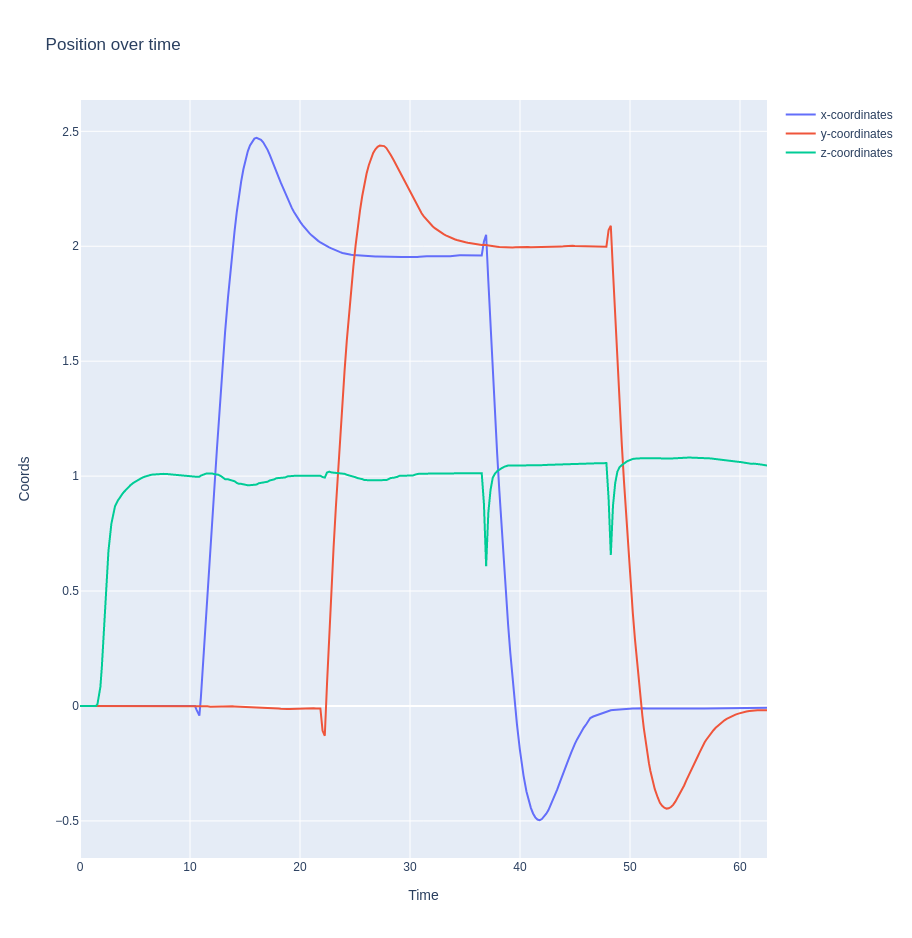
\includegraphics[width=1.0\linewidth]{images/task2_sim_pos.png}
	\caption{x, y and z coordinates of the drone in simulation. ($K_p = 0.1$, $K_i = 0.01$, $K_d = 0.1$)}
	\label{fig:sim_pos}
\end{figure}

Another way to visualize the simulation is using the program rviz which makes is possible to display the orientation as well as the position in 3D space. This can be seen on \cref{fig:sim_rviz}. On this figure it is also apparent that the yaw angle is constant for the drone at all times. When observing the behaviour on \cref{fig:sim_rviz} the controller was again verified to be a good start for the real world scenario.

\begin{figure}[hbtp]
	\centering
	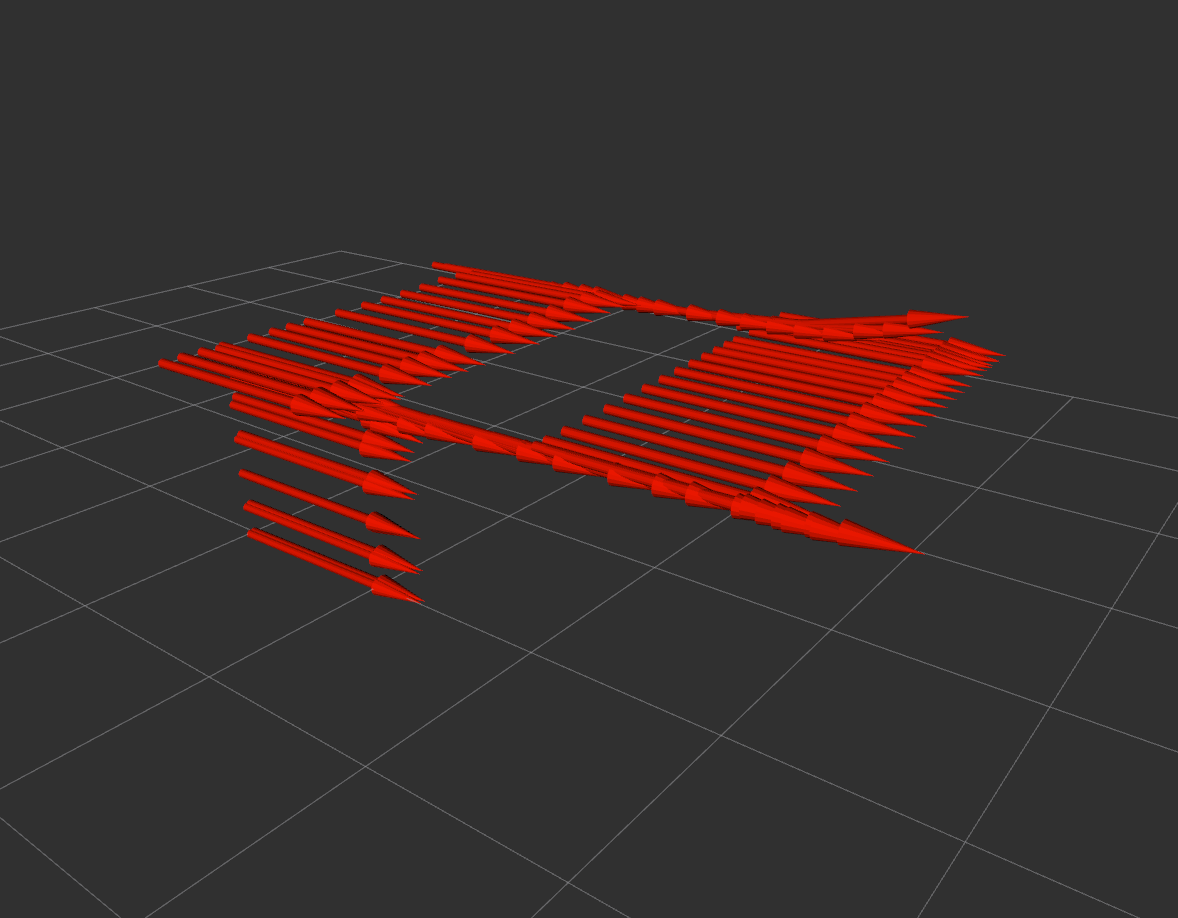
\includegraphics[width=1.0\linewidth]{images/task2_sim_rviz.png}
	\caption{x, y and z coordinates of the drone in simulation. ($K_p = 0.1$, $K_i = 0.01$, $K_d = 0.1$)}
	\label{fig:sim_rviz}
\end{figure}

\subsection{Real world results}
After having tested the controller in simulation the next step is to test it in a real world scenario. This is done using the Vicon motion control system which is able to accurately measure a UAV's position. This is done through 12 motion capture cameras that can locate small grey balls which are taped onto the drone itself. The Vicon system uses these balls as an reference point in space which can then be grouped together in the Vicon software and it will be able to publish the position as a topic in ROS. This means that the controller will now subscribe to this topic instead of the odometry data from the UAV itself.

\textbf{Task 1}
The first task is to get the UAV to hover and be able to withstand disturbances. This means, in a real world scenario, if the drone experiences large gushes of wind it will be able to go back to its original position autonomously. To simulate this disturbance a piece of string was tied to the UAV and a person would simply pull in the string.

On \cref{fig:task1_10_pos} the drone is set to hover at position (0, 0, 1). The controller is the same as in simulation ($K_p = 0.1$, $K_i = 0.01$, $K_d = 0.1$). It can be seen how the UAV flies to the desired location and then a big disturbance occurs which displaces the UAV over 2.5 meters in the negative x-direction. However the UAV quickly recovers and converges to its original position.  

\begin{figure}[hbtp]
	\centering
	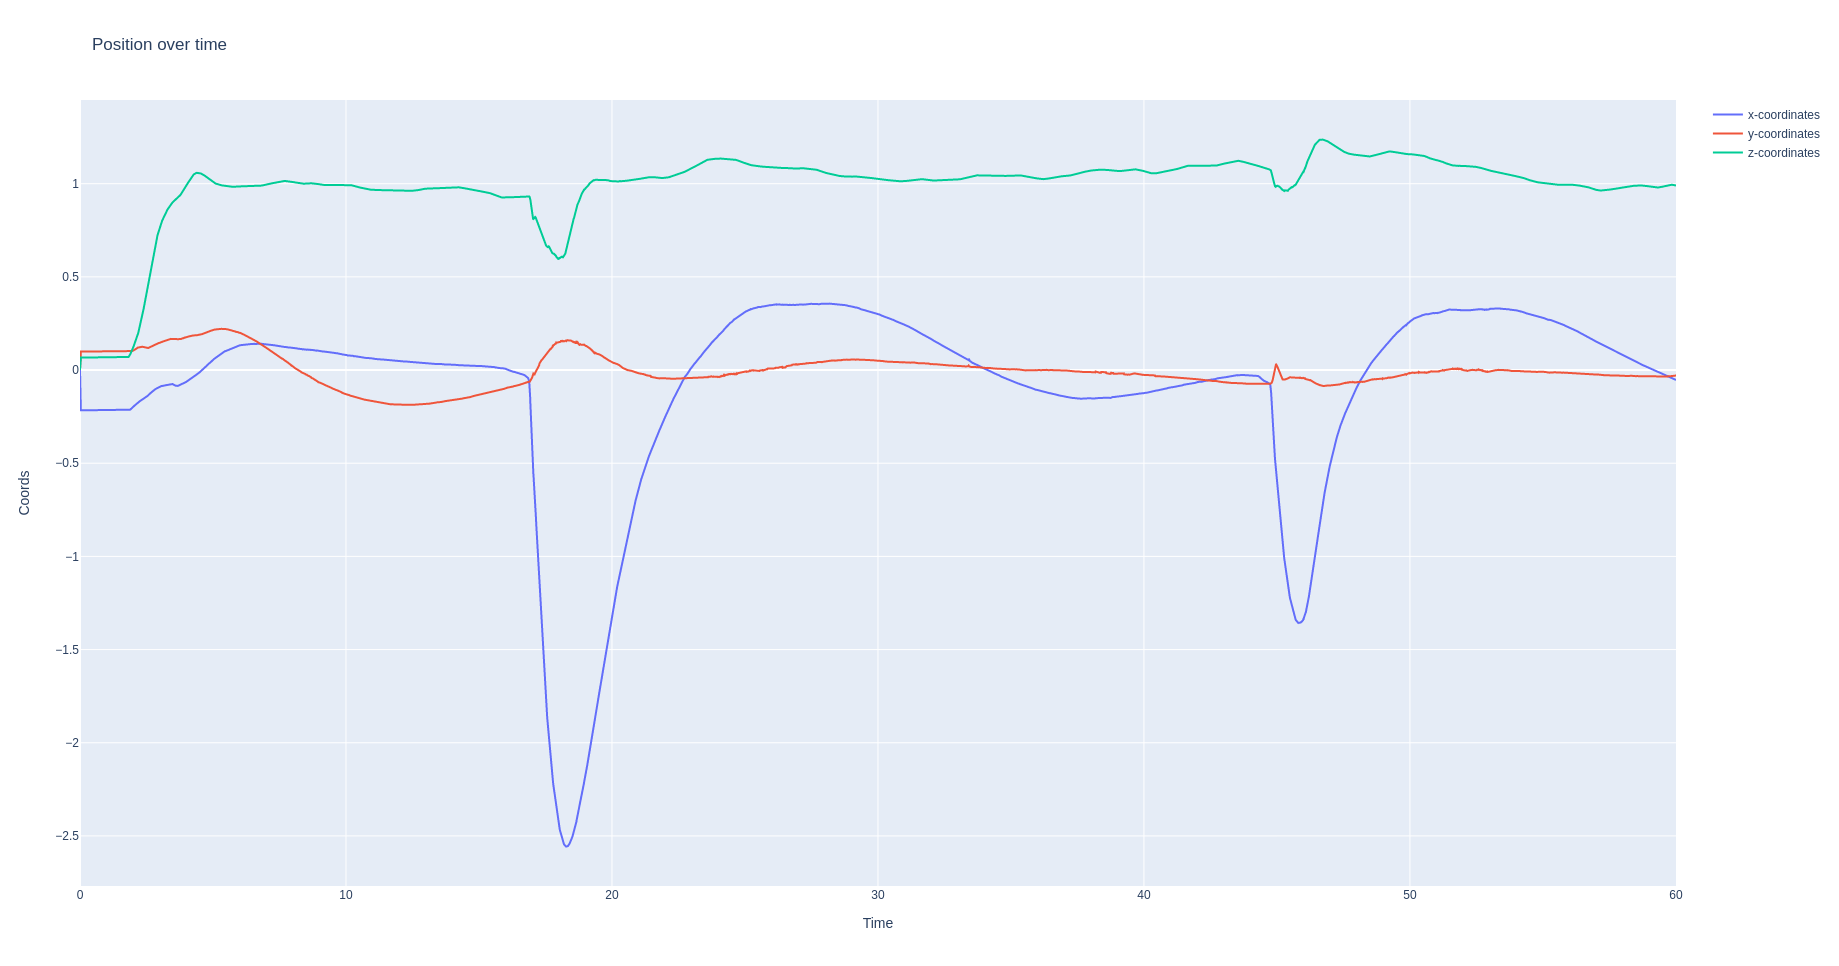
\includegraphics[width=1.0\linewidth]{images/task1_10_pos.png}
	\caption{x, y and z coordinates of the UAV in the hovering scenario. ($K_p = 0.1$, $K_i = 0.01$, $K_d = 0.1$)}
	\label{fig:task1_10_pos}
\end{figure}

On \cref{fig:task1_10_err} the same behaviour can be seen. When the disturbance occurs there is a big spike in the error which is expected. 

\begin{figure}[hbtp]
	\centering
	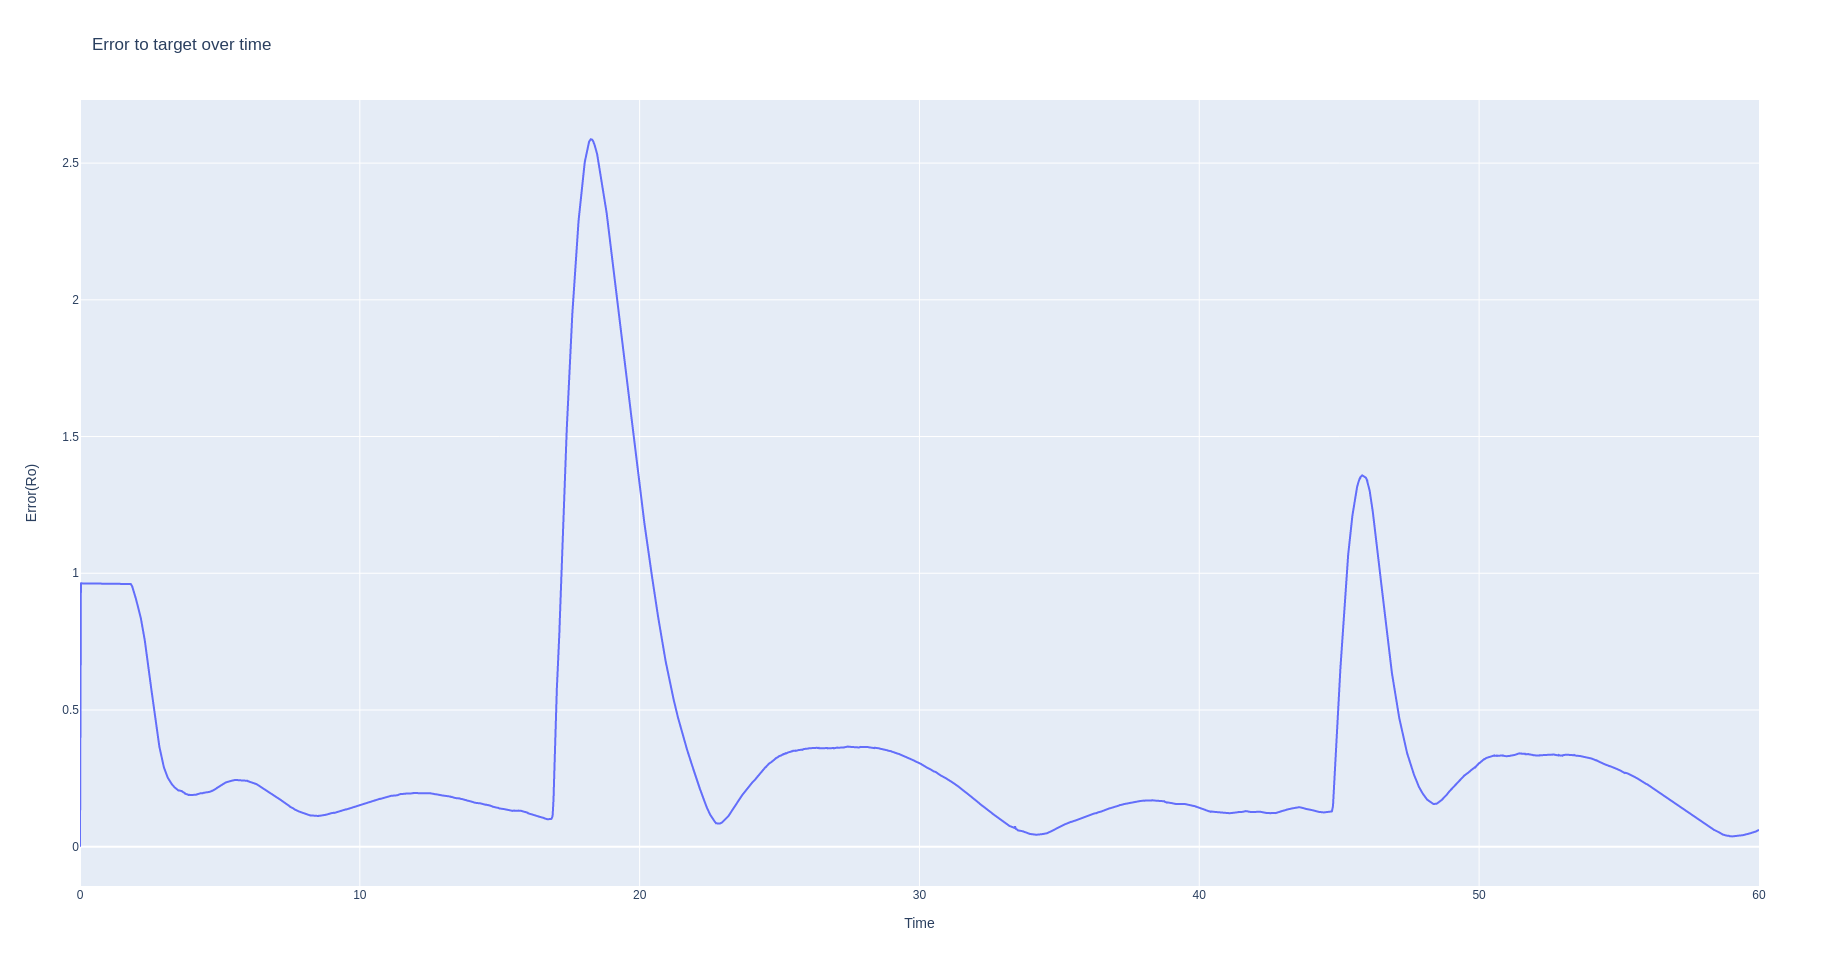
\includegraphics[width=1.0\linewidth]{images/task1_10_err.png}
	\caption{Error(distance) to target(0,0,1). ($K_p = 0.1$, $K_i = 0.01$, $K_d = 0.1$)}
	\label{fig:task1_10_err}
\end{figure}

The controller used on \cref{fig:task1_10_err} and \cref{fig:task1_10_pos} seems to be doing a good job, however it also looks like it can be improved. By tuning the value of Kd the overshoot should decrease and in turn make it settle quicker which is one of the requirements for this controller. On \cref{fig:task1_11_pos} the position of the UAV can be seen. $K_d$ has been increase threefold and now the overshoot has decreased greatly and it settles quicker. It still looks like there is some overshoot but it was observed during the test that the string attached to the UAV cause some amount of drag and made the UAV move slightly slower causing this overshoot from t=25 to t=43.

\begin{figure}[hbtp]
	\centering
	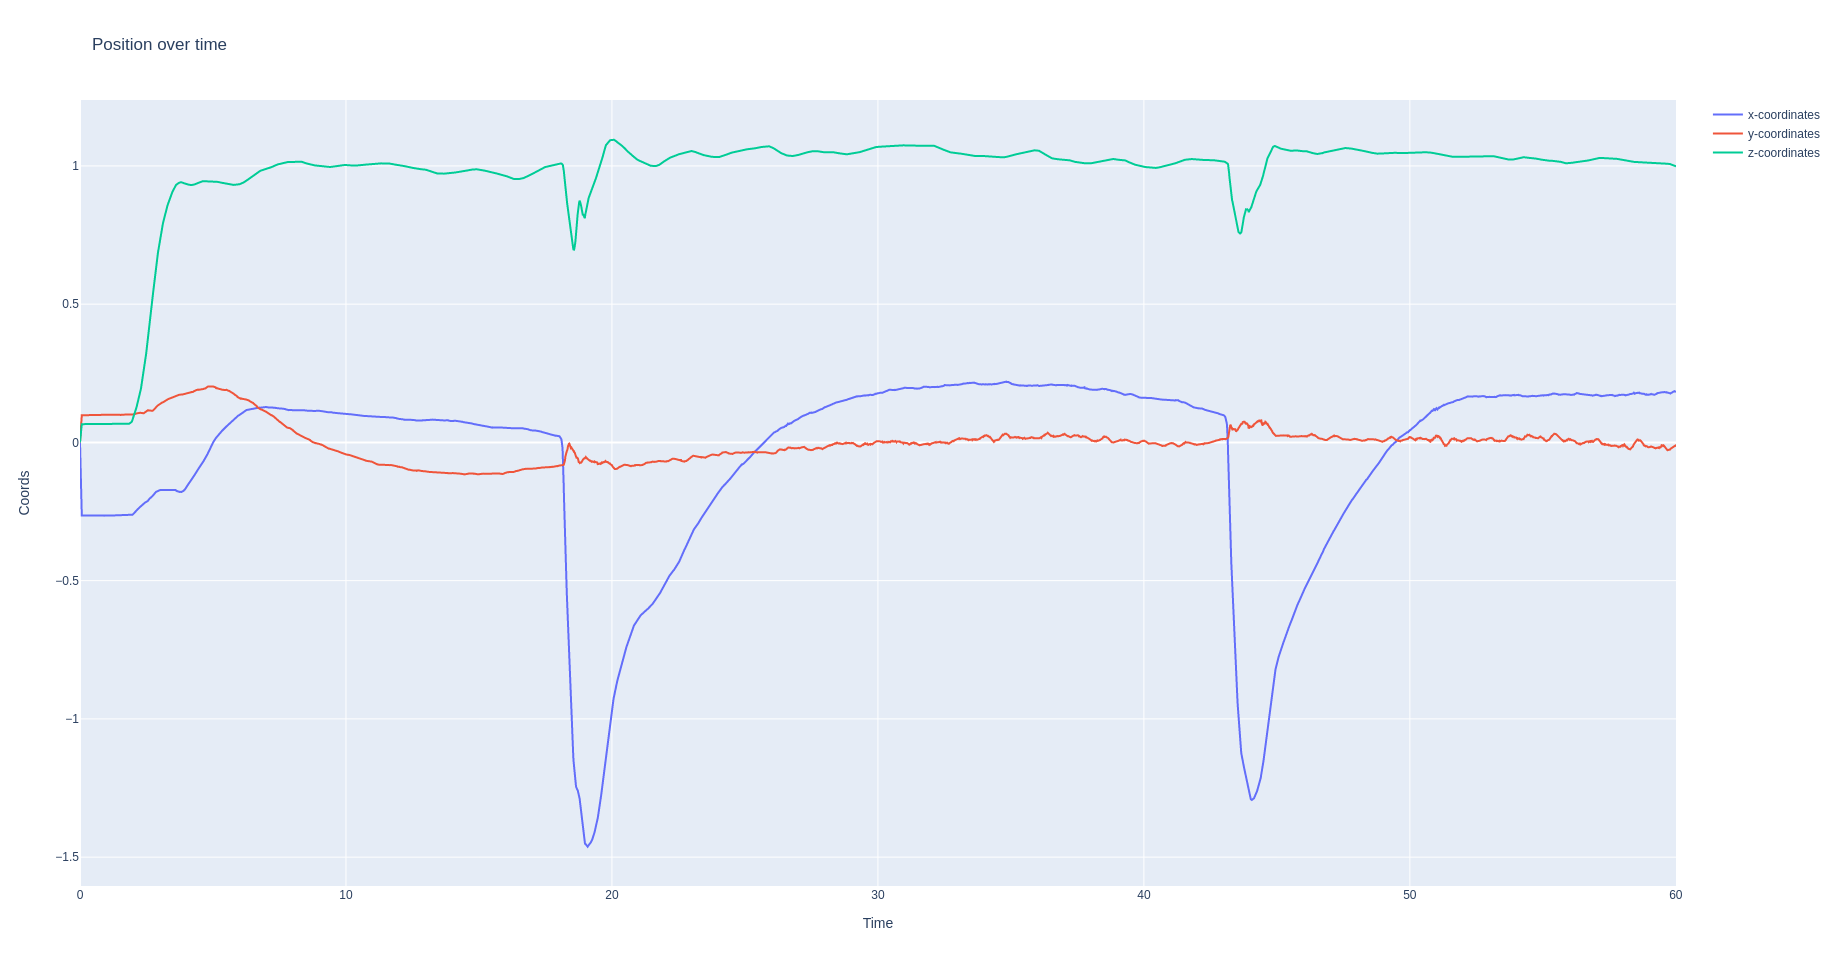
\includegraphics[width=1.0\linewidth]{images/task1_11_pos.png}
	\caption{x, y and z coordinates of the UAV. ($K_p = 0.1$, $K_i = 0.01$, $K_d = 0.3$)}
	\label{fig:task1_11_pos}
\end{figure}

On \cref{fig:task1_11_err} the error to the target can be seen. It shows the same drawn out overshoot caused by the strings weight and drag on the floor.

\begin{figure}[hbtp]
	\centering
	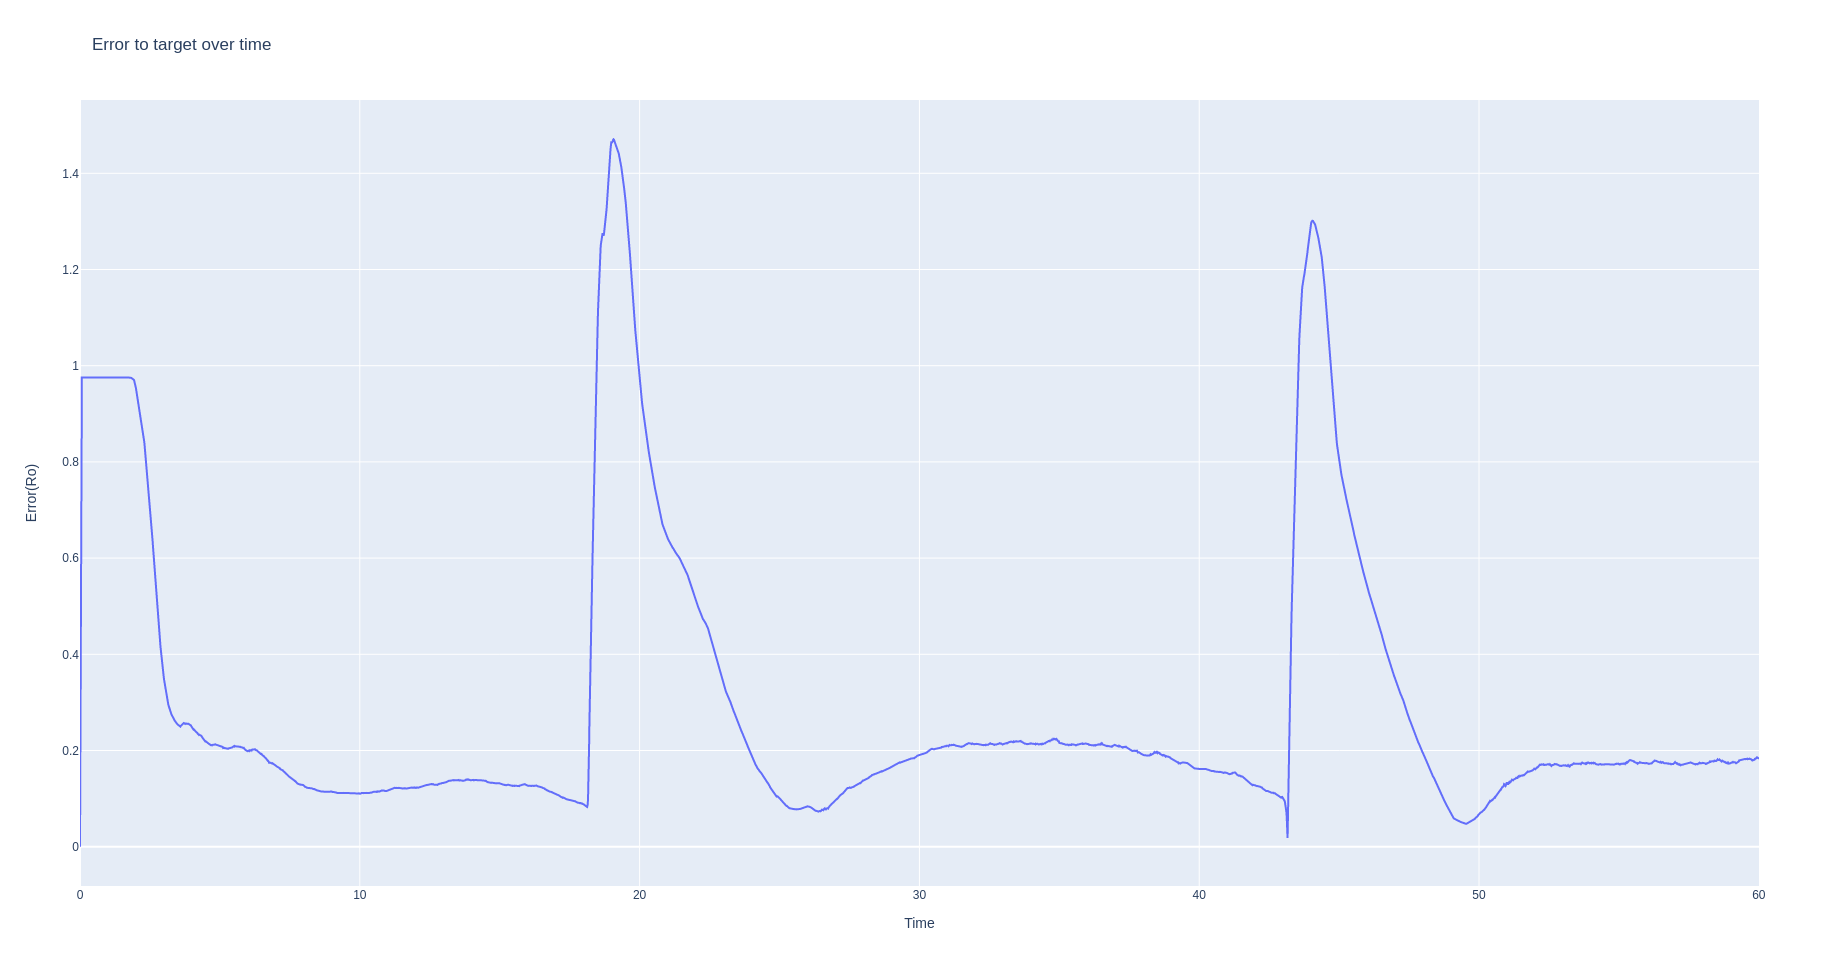
\includegraphics[width=1.0\linewidth]{images/task1_11_err.png}
	\caption{Error(distance) to target(0,0,1). ($K_p = 0.1$, $K_i = 0.01$, $K_d = 0.3$)}
	\label{fig:task1_11_err}
\end{figure}

To decrease the rise time and eliminate the steady state error an increase in $K_i$ will help alleviate that. This comes with a cost of an increase in settling time and decreases the stability which goes against the requirements for this controller. A controller with a $Ki=0.03$ has been tested and shows that the UAV takes a big hit to the settling time. These figures can be seen in appendix A.

When tuning the proportional term of the controller the rise time should decrease and the overshoot should increase, however the settling time will increase and the stability will decrease. On \cref{fig:task1_4_pos} it can be seen how the overshoot is increase compared to \cref{fig:task1_10_pos} and the stability has been decreased. 

\begin{figure}[hbtp]
	\centering
	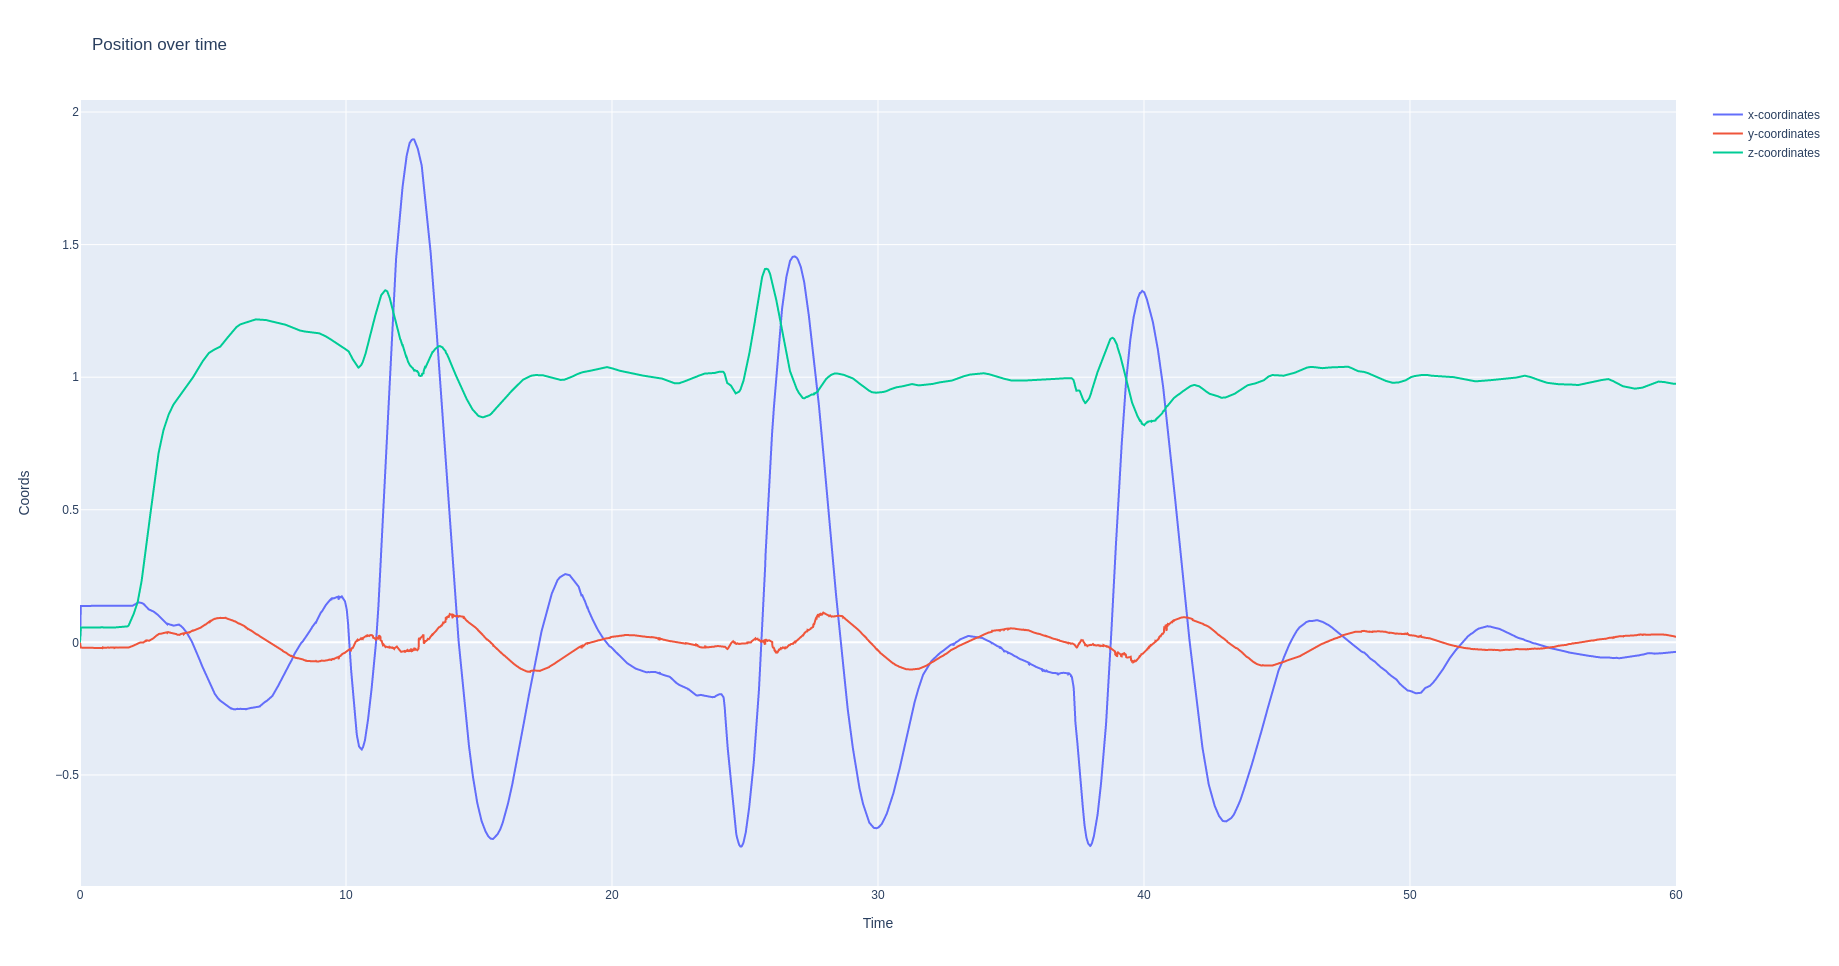
\includegraphics[width=1.0\linewidth]{images/task1_4_pos.png}
	\caption{x, y and z coordinates of the UAV. ($K_p = 0.3$, $K_i = 0.01$, $K_d = 0.1$)}
	\label{fig:task1_4_pos}
\end{figure}

The overshoot and stability issues can also be seen on \cref{fig:task1_4_err}. 
\begin{figure}[hbtp]
	\centering
	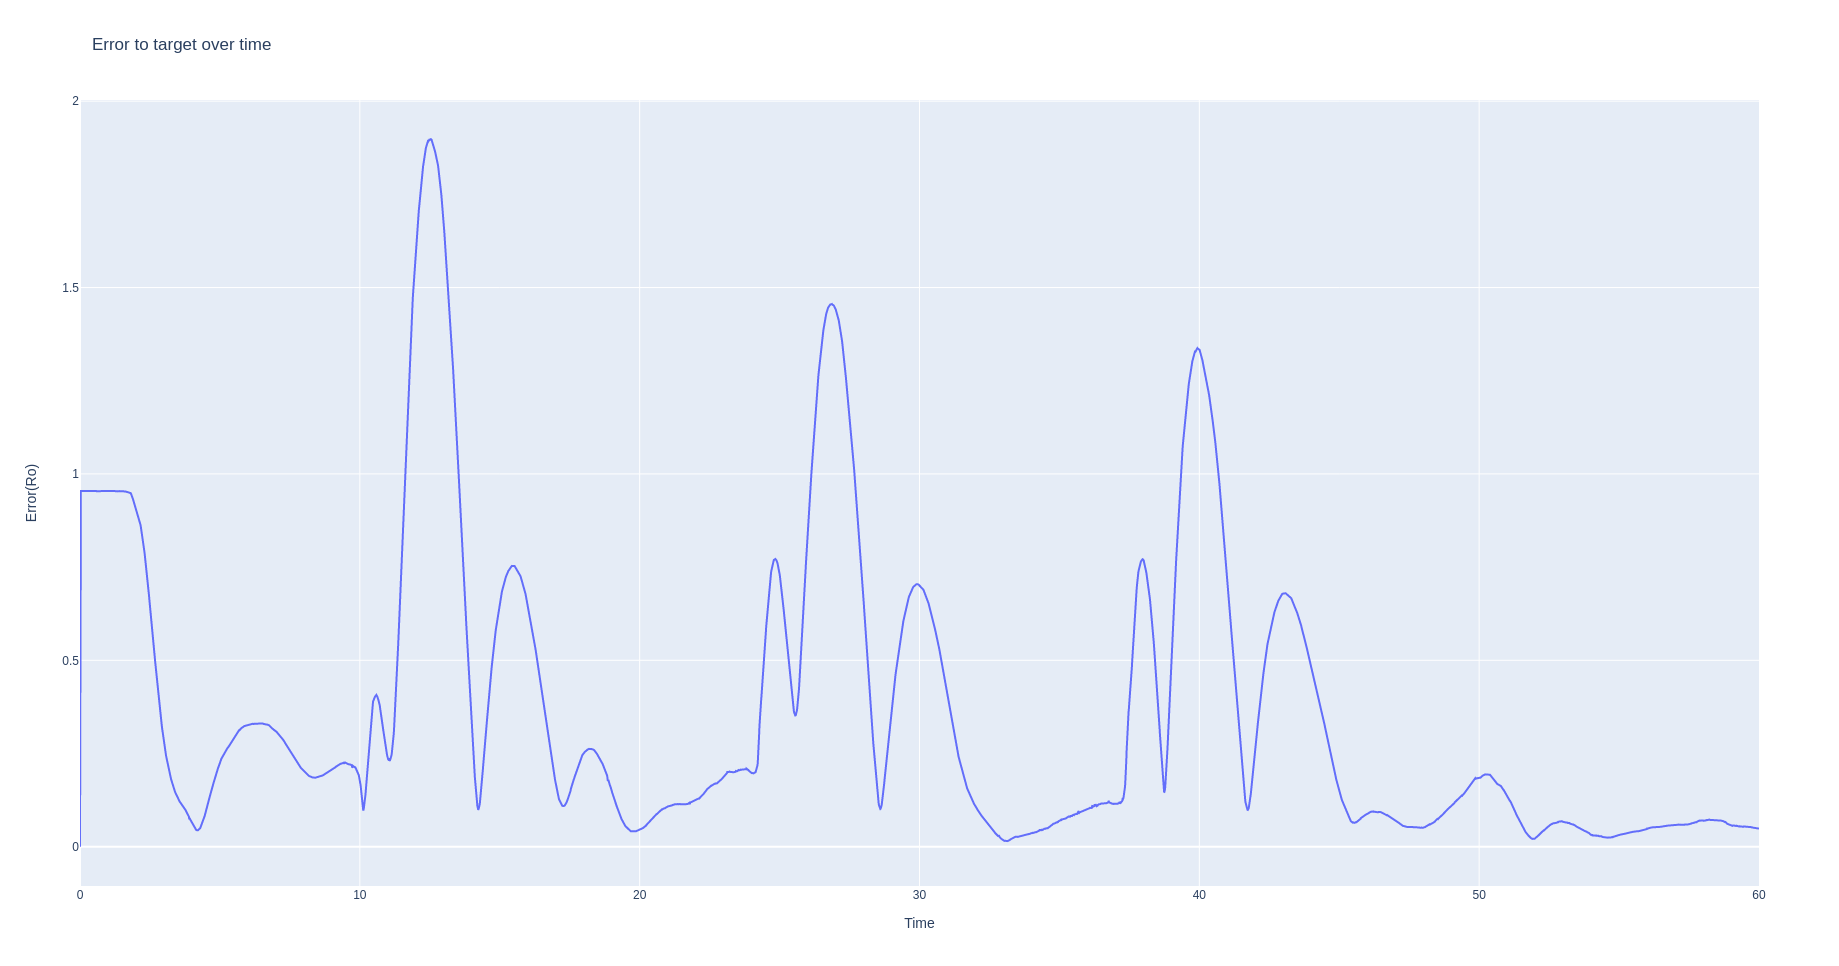
\includegraphics[width=1.0\linewidth]{images/task1_4_err.png}
	\caption{Error(distance) to target(0,0,1). ($K_p = 0.3$, $K_i = 0.01$, $K_d = 0.3$)}
	\label{fig:task1_4_err}
\end{figure}

After looking at all of these plots where each controller parameter has been examined individually, it has given a much more intuitively understanding of what effect each controller parameter has on the output. THis gives the basis of manual tuning the optimal PID-controller for the task. After some manual tuning the parameters for this controller was found to be $K_p = 0.4$, $K_i = 0.02$, $K_d = 0.4$. By using the proportional, integral and derivative part it is possible to cancel out the negative aspects of each term. This controller can be seen on \cref{fig:task1_9_pos}. There is a significant amount of jitter when looking at the y-axis. This was observed in multiple tests and only occurred when the UAV was in a certain location. This could indicate a problem with the Vicon system or a problem with the motion capture system unable to locate all the balls taped onto the UAV. Whenever the UAV moved out this area the jitter disappeared and it performed as expected. This jitter can be seen on \cref{fig:task1_9_pos} and \cref{fig:task1_9_err} at t=15 and t=35.

\begin{figure}[hbtp]
	\centering
	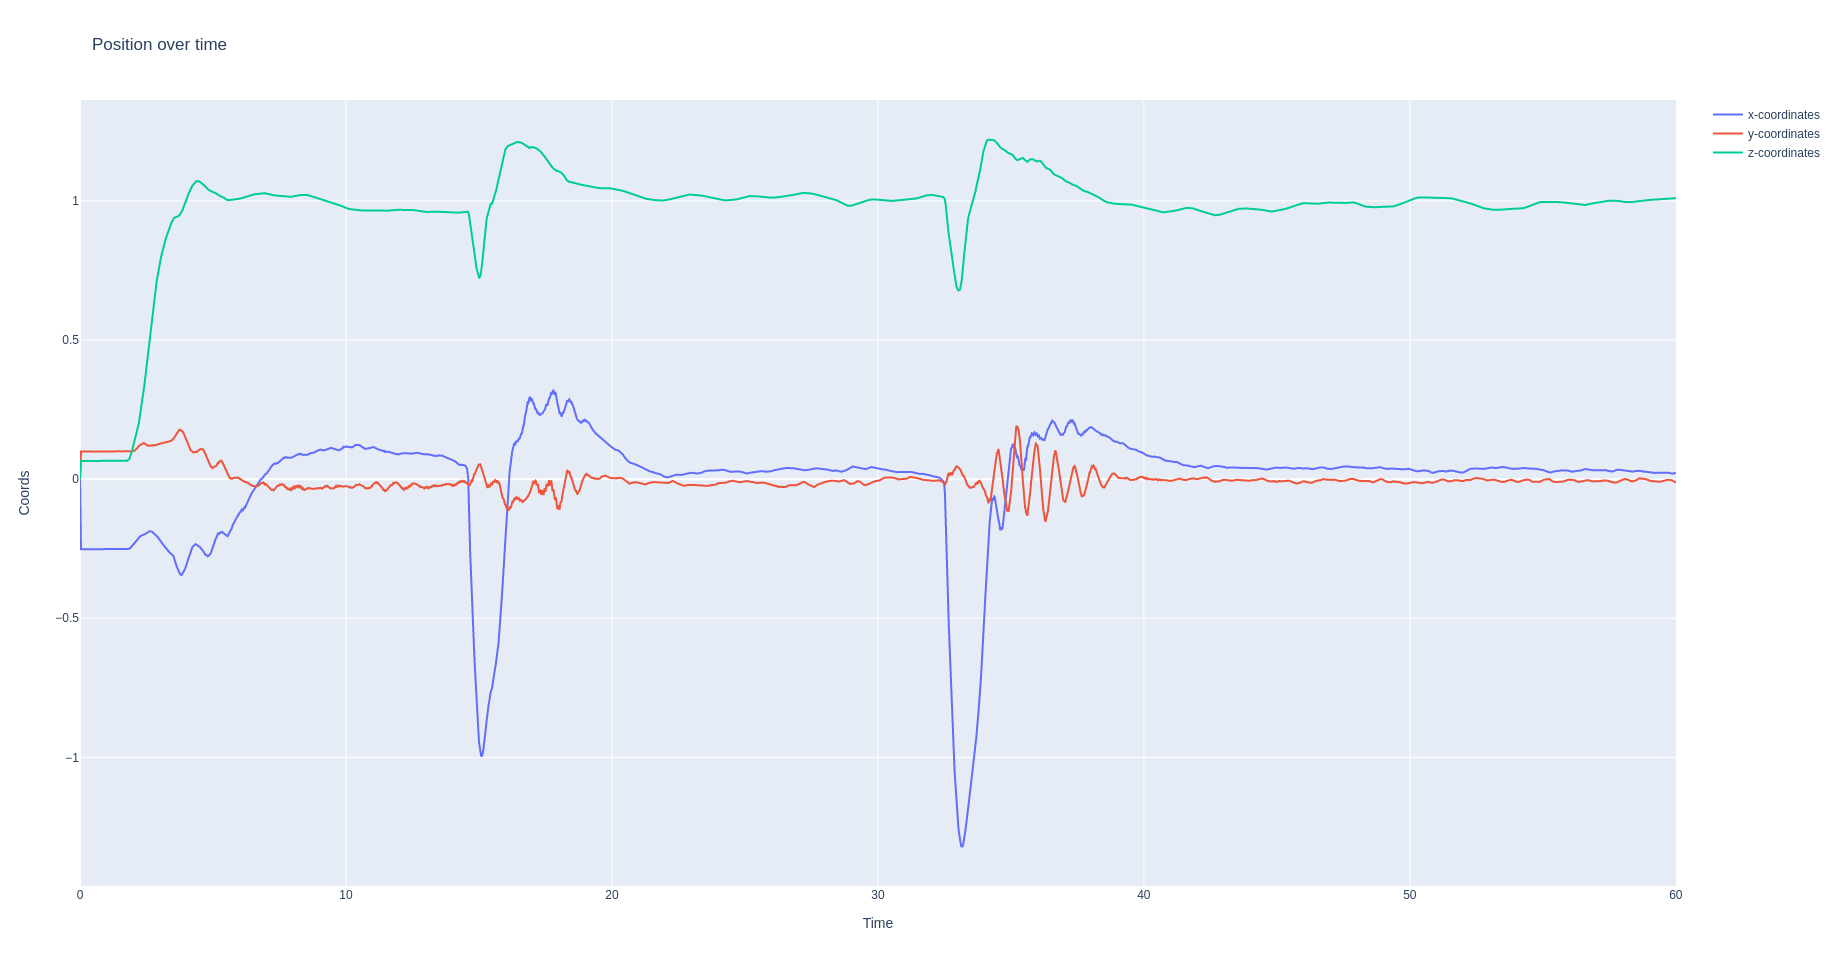
\includegraphics[width=1.0\linewidth]{images/task1_9_pos.png}
	\caption{x, y and z coordinates of the UAV. ($K_p = 0.4$, $K_i = 0.02$, $K_d = 0.4$)}
	\label{fig:task1_9_pos}
\end{figure}

\begin{figure}[hbtp]
	\centering
	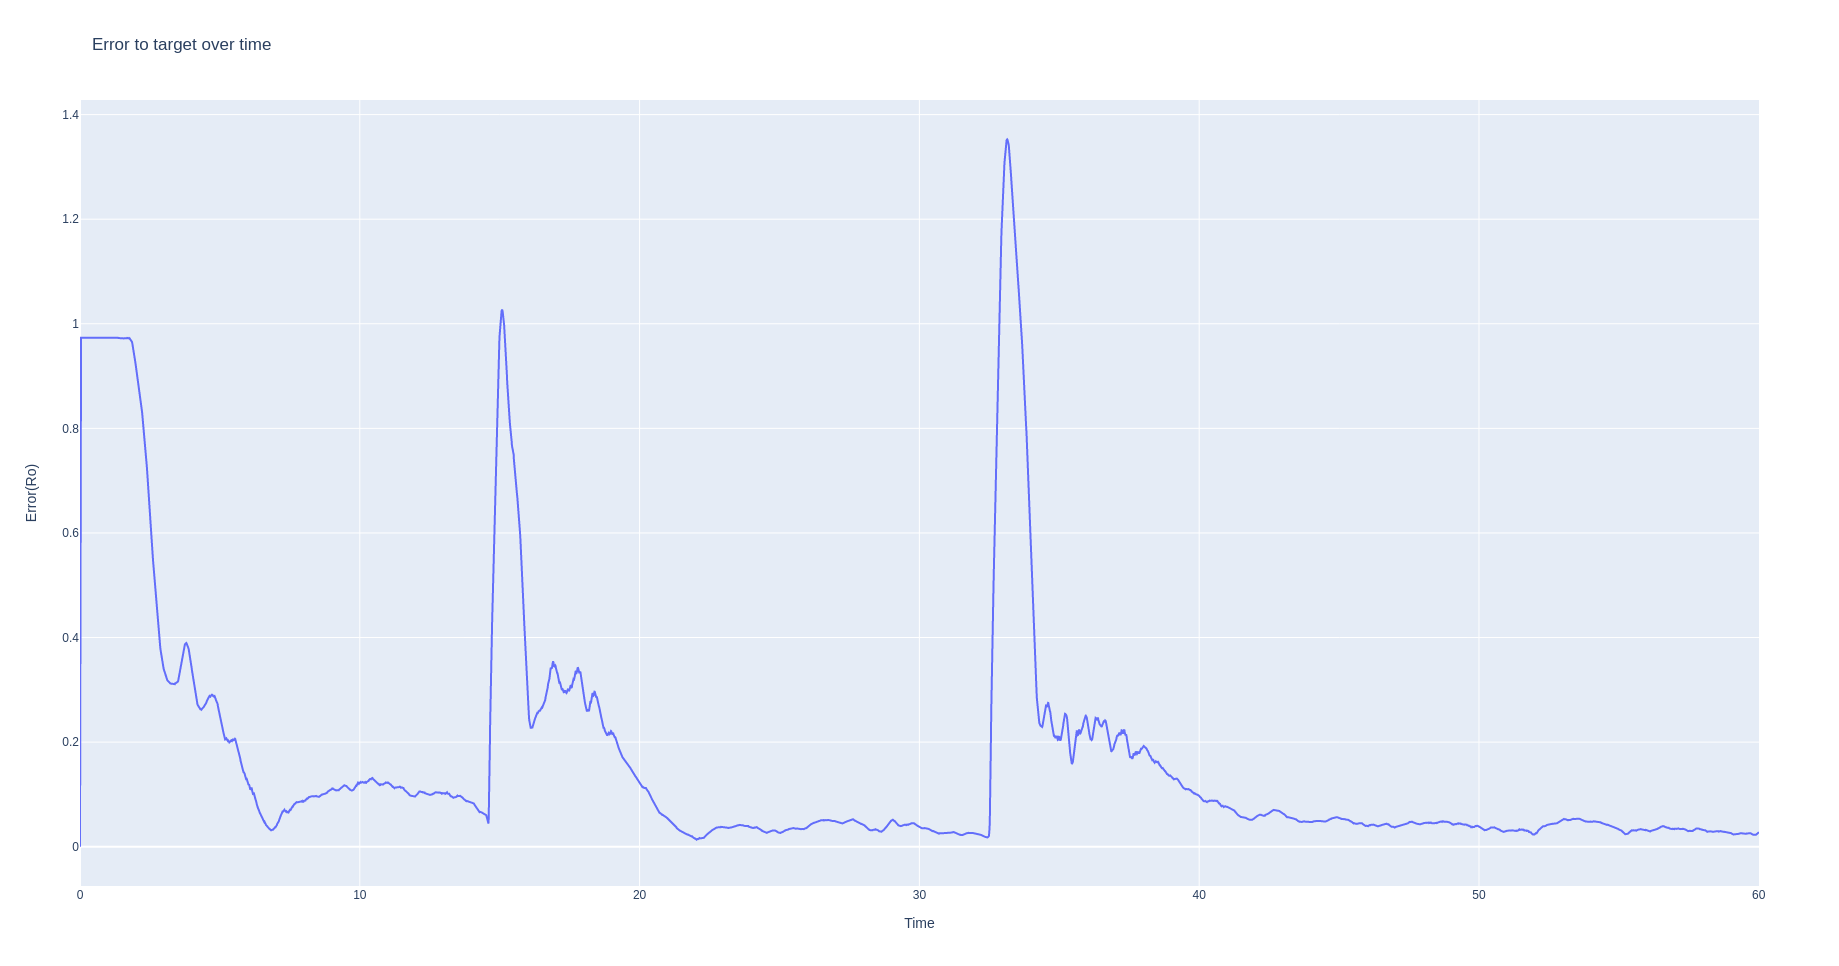
\includegraphics[width=1.0\linewidth]{images/task1_9_err.png}
	\caption{x, y and z coordinates of the UAV. ($K_p = 0.4$, $K_i = 0.02$, $K_d = 0.4$)}
	\label{fig:task1_9_err}
\end{figure}

Based on the last two figures a very quick and stable controller has been made and it meets the requirement of having a quick settling time.

\textbf{Task 2}

The objective of task 2 were to make the UAV fly autonomously in square shape trajectory by visiting four user defined way-points using a PID-controller with an arbitrary yaw angle. Further more different settings for the PID-controller should be tested and analyzed. The UAV has to wait at a way-point for at least 3 seconds before flying on to the next one. 
The chosen coordinates for the four way-points are (2,0,1), (2,2,1), (0,2,1) and (0,0,1), which forms a square shape one meter above the ground. Like in task 1 were the controller tested in the simulation chosen as base controller with the controller parameters of $K_p = 0.1$, $K_i = 0.01$, $K_d = 0.1$. On \cref{fig:task2_1_pos} and \cref{fig:task2_1_err} can the results of the UAV with a base PID-controller implemented visiting the 4 way-point be seen.
On \cref{fig:task2_1_pos} the x, y and z position of the UAV over time can be seen and on \cref{fig:task2_1_err} the error to the next way-point can be seen. 


\begin{figure}[hbtp]
	\centering
	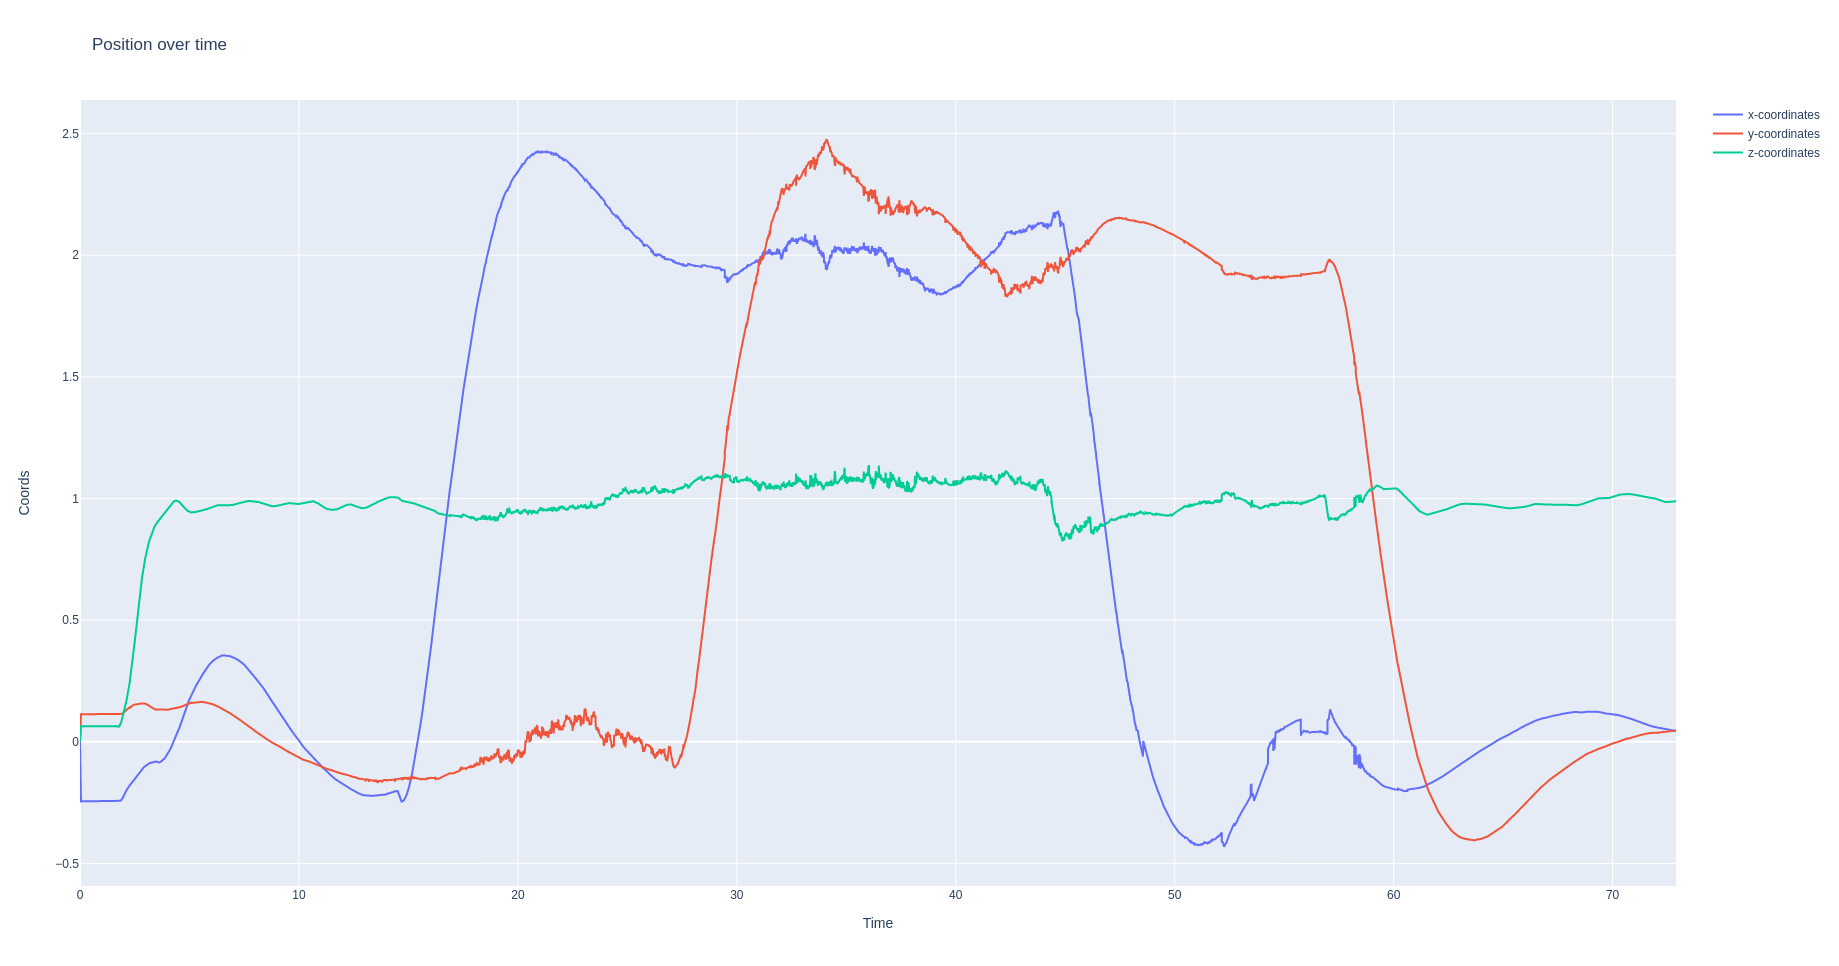
\includegraphics[width=1.0\linewidth]{images/task2_1_pos.png}
	\caption{x, y and z coordinates of the UAV. ( $K_p = 0.1$, $K_i = 0.01$, $K_d = 0.1$)}
	\label{fig:task2_1_pos}
\end{figure}

\begin{figure}[hbtp]
	\centering
	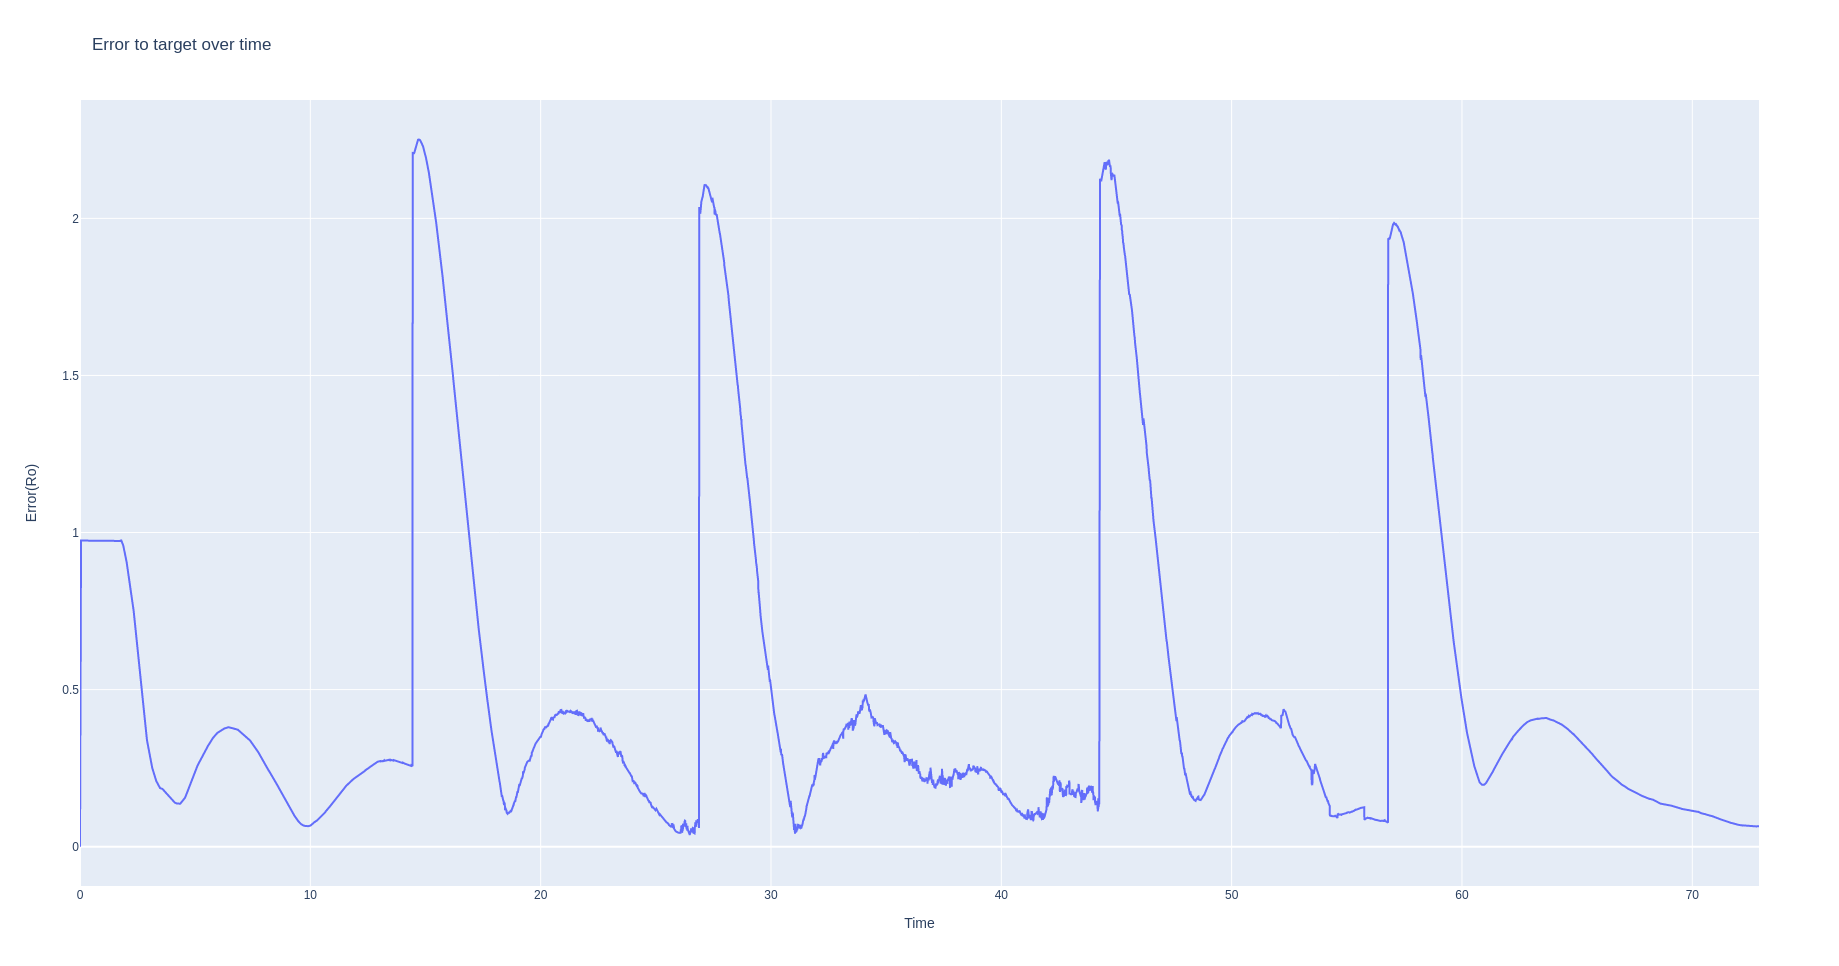
\includegraphics[width=1.0\linewidth]{images/task2_1_err.png}
	\caption{Error(distance) to way-points. ( $K_p = 0.1$, $K_i = 0.01$, $K_d = 0.1$)}
	\label{fig:task2_1_err}
\end{figure}

\cref{fig:task2_1_pos} and \cref{fig:task2_1_err} shows how the UAV flies rather quickly on to the next way-point where it makes an overshoot around 20-25\%. 
Like task 1 $K_d$ is now increased so the slope of the change of error over time should have a bigger weight in the controller output. This will translate to a decrease in overshoot. On \cref{fig:task2_4_pos} and \cref{fig:task2_4_err} the result of controller parameter $K_d$ is increased to 0.3 and $K_p$ and $K_i$ remains the same. 


\begin{figure}[hbtp]
	\centering
	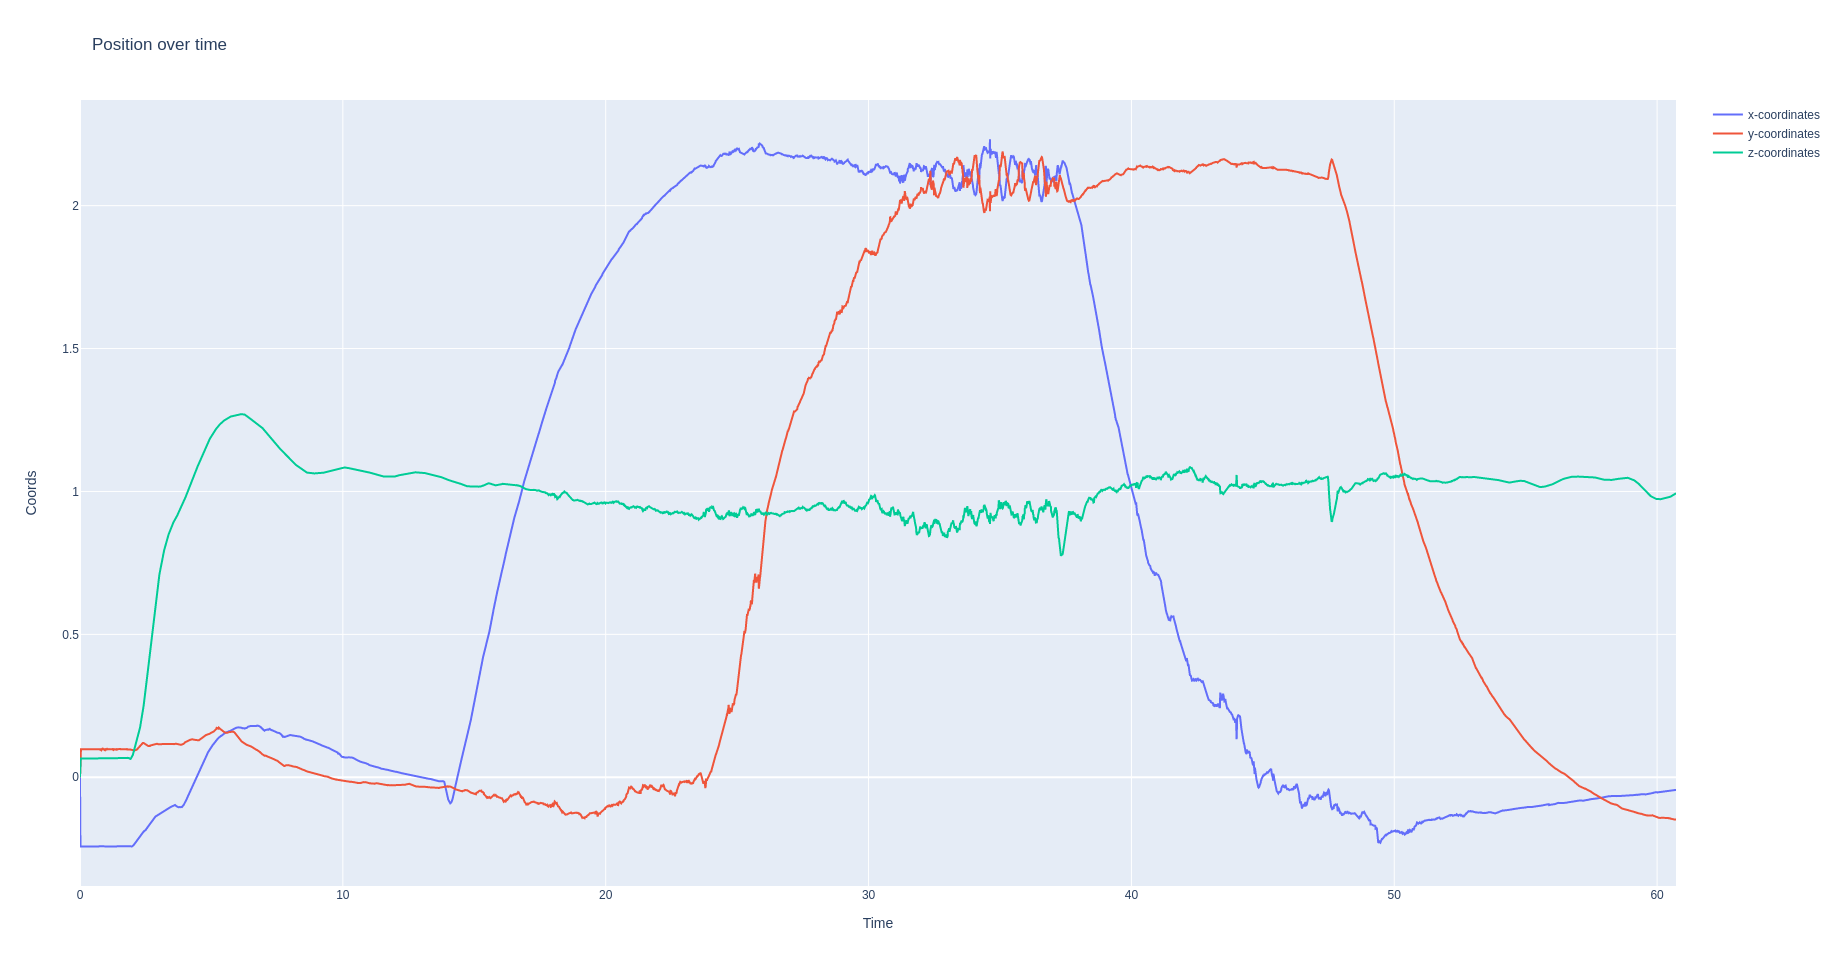
\includegraphics[width=1.0\linewidth]{images/task2_4_pos.png}
	\caption{x, y and z coordinates of the UAV. ( $K_p = 0.1$, $K_i = 0.01$, $K_d = 0.3$)}
	\label{fig:task2_4_pos}
\end{figure}

\begin{figure}[hbtp]
	\centering
	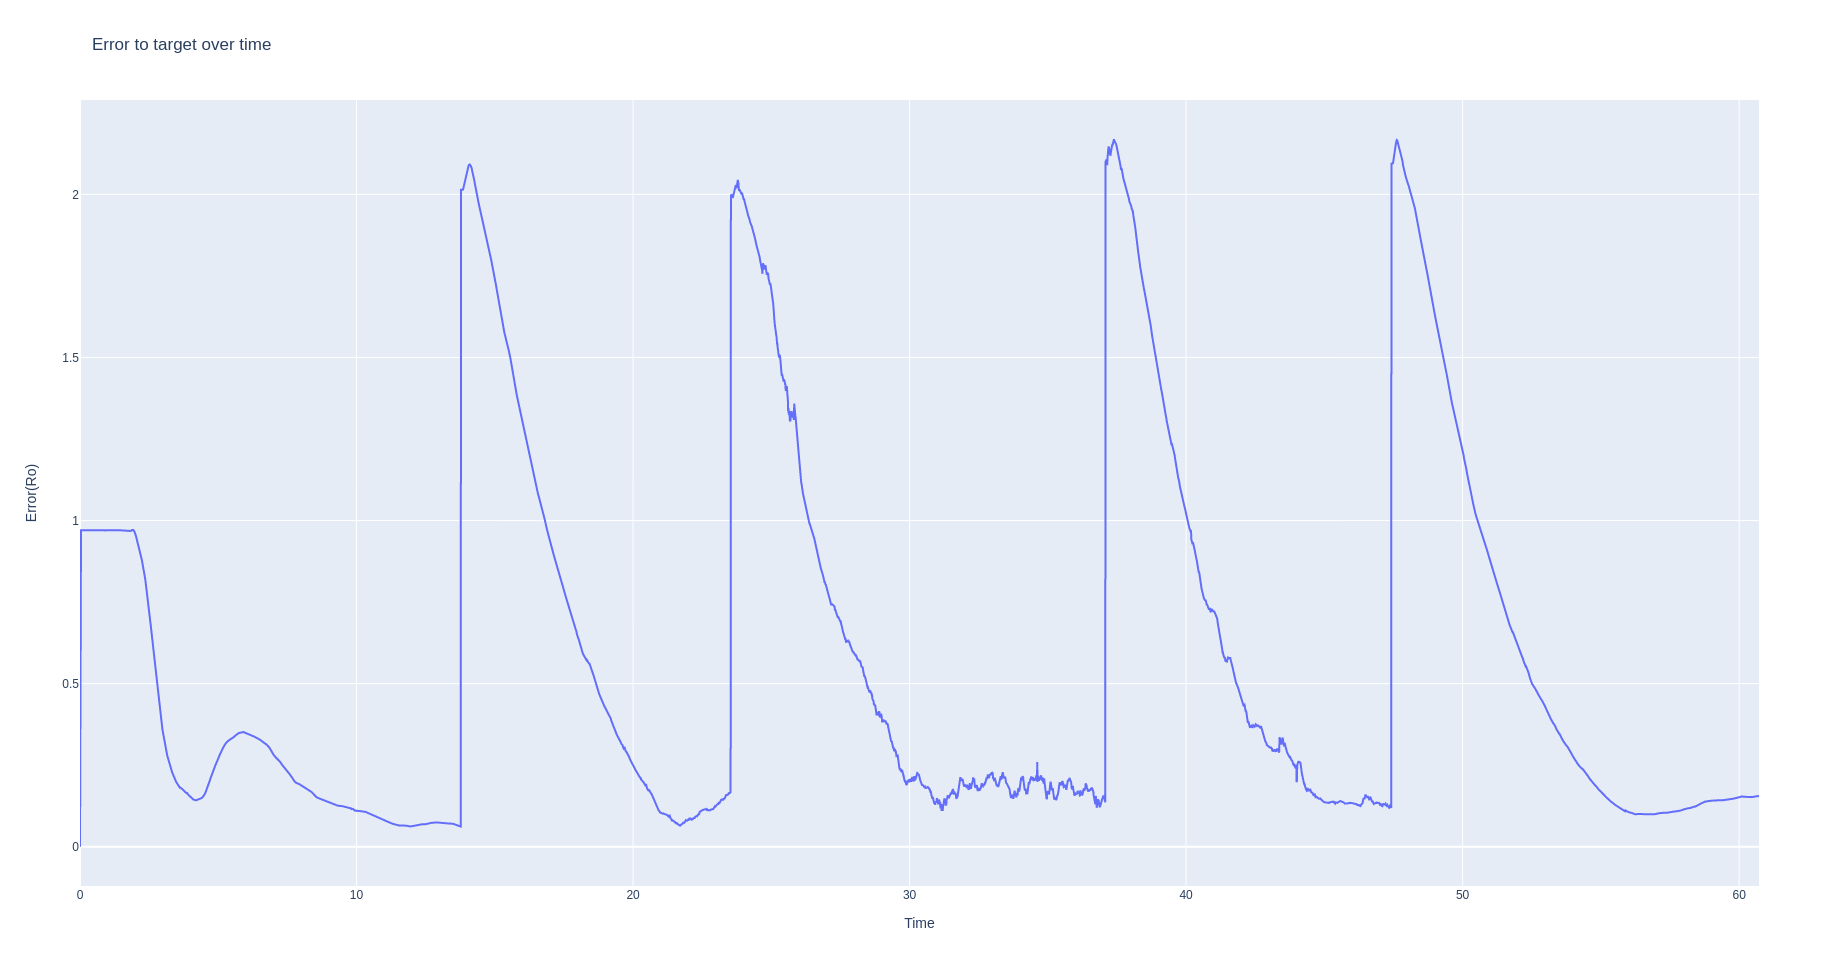
\includegraphics[width=1.0\linewidth]{images/task2_4_err.png}
	\caption{Error(distance) to way-points. ( $K_p = 0.1$, $K_i = 0.01$, $K_d = 0.3$)}
	\label{fig:task2_4_err}
\end{figure}

As expected, the overshoot decrease and it actually disappeared. On the downside the UAV is not as quick  and the rise time has increased. The is because the slope of the change of error over time has a bigger influence on the controller output, which means if the UAV approaches the next way-point quickly the will slope be more negative resulting in a lower controller output. 
Next is the controller parameter $K_i$ increased and $K_d$ is changed back to 0.1. This should result in a increase in rise time and overshoot. On \cref{fig:task2_3_pos} and \cref{fig:task2_3_err} the controller parameter $K_i$ is increased to 0.03 and $K_p$ and $K_d$ are both 0.1. 

\begin{figure}[hbtp]
	\centering
	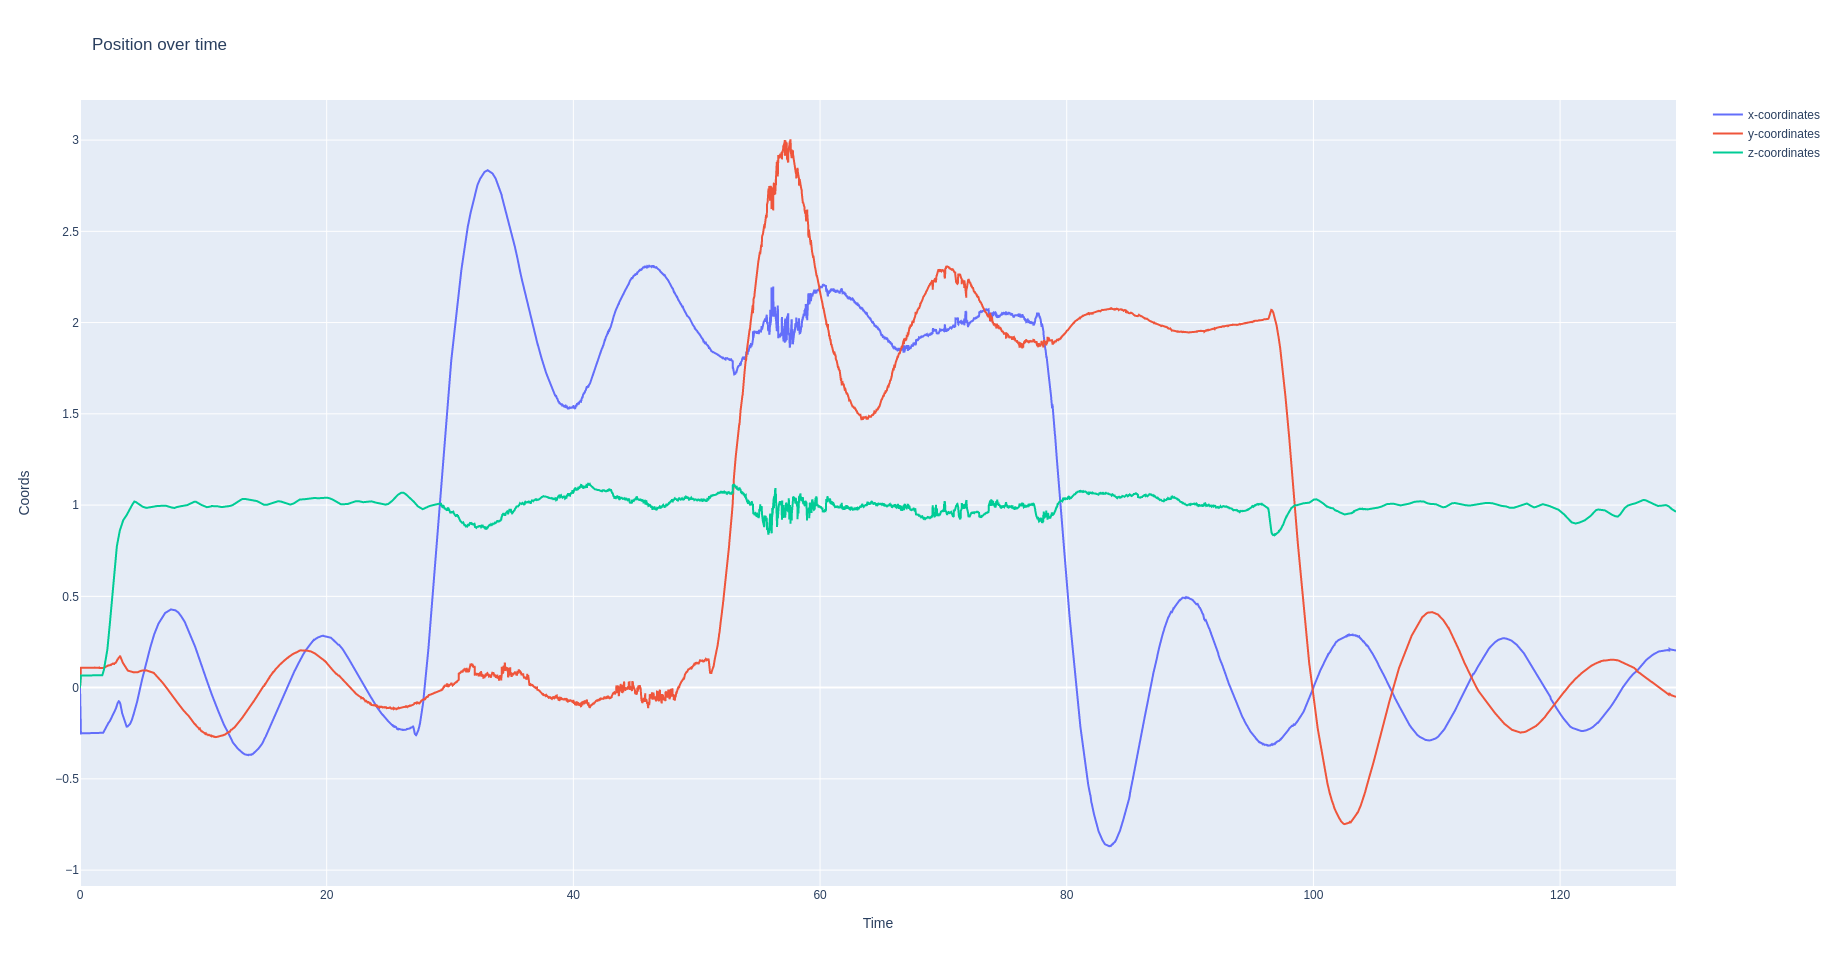
\includegraphics[width=1.0\linewidth]{images/task2_3_pos.png}
	\caption{x, y and z coordinates of the UAV. ( $K_p = 0.1$, $K_i = 0.03$, $K_d = 0.1$)}
	\label{fig:task2_3_pos}
\end{figure}

\begin{figure}[hbtp]
	\centering
	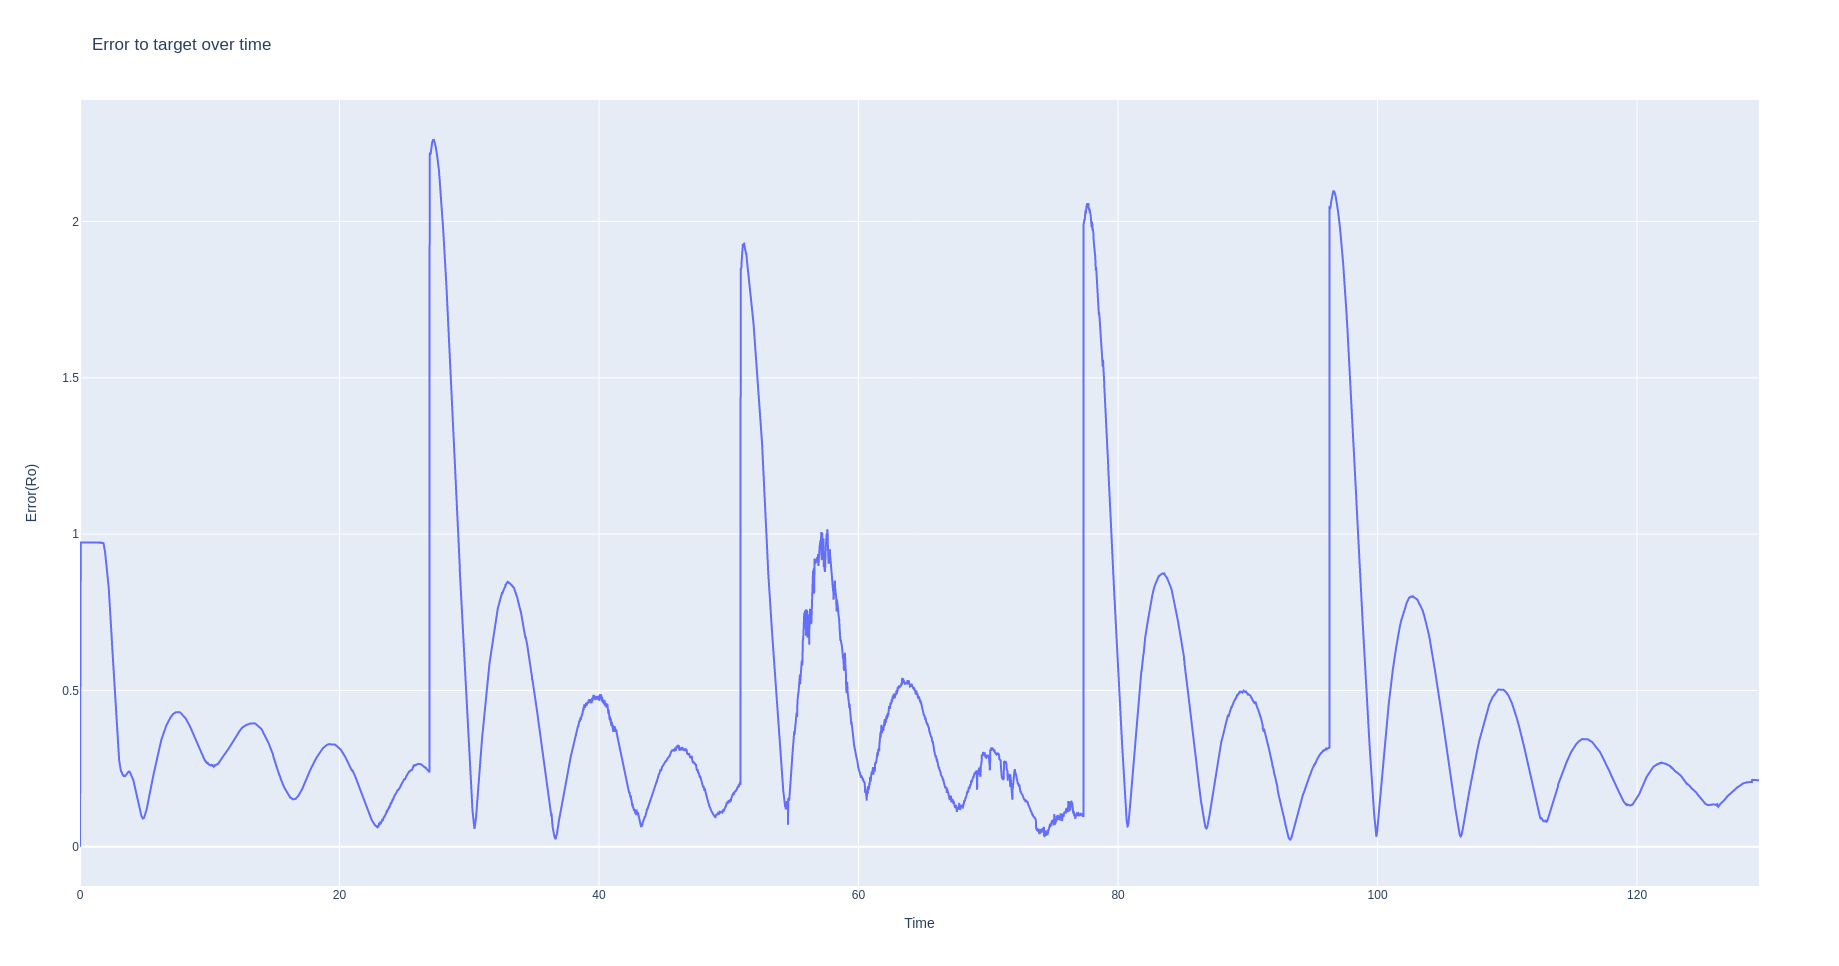
\includegraphics[width=1.0\linewidth]{images/task2_3_err.png}
	\caption{Error(distance) to way-points. ( $K_p = 0.1$, $K_i = 0.03$, $K_d = 0.1$)}
	\label{fig:task2_3_err}
\end{figure}

As expected the UAV is now flying much faster to next way-point compared to when $K_d$ was increased. On the other hand overshoot has been increased to almost 45\% and the settling time is very high as well. This is because an increase in $K_i$ makes past error have a bigger influence on the controller output and as the accumulated error first becomes smaller after the goal has been reached the UAV will tend to overshoot more and increase settling time. 
In the last test before making the optimal controller the controller parameter $K_p$ will be increased and $K_i$ will be changed back to 0.01. On \cref{fig:task2_4_pos} and \cref{fig:task2_4_err} the result of the controller parameter $K_p$ is increased to 0.3 and $K_i$ is 0.01 and $K_d$ is 0.1.

\begin{figure}[hbtp]
	\centering
	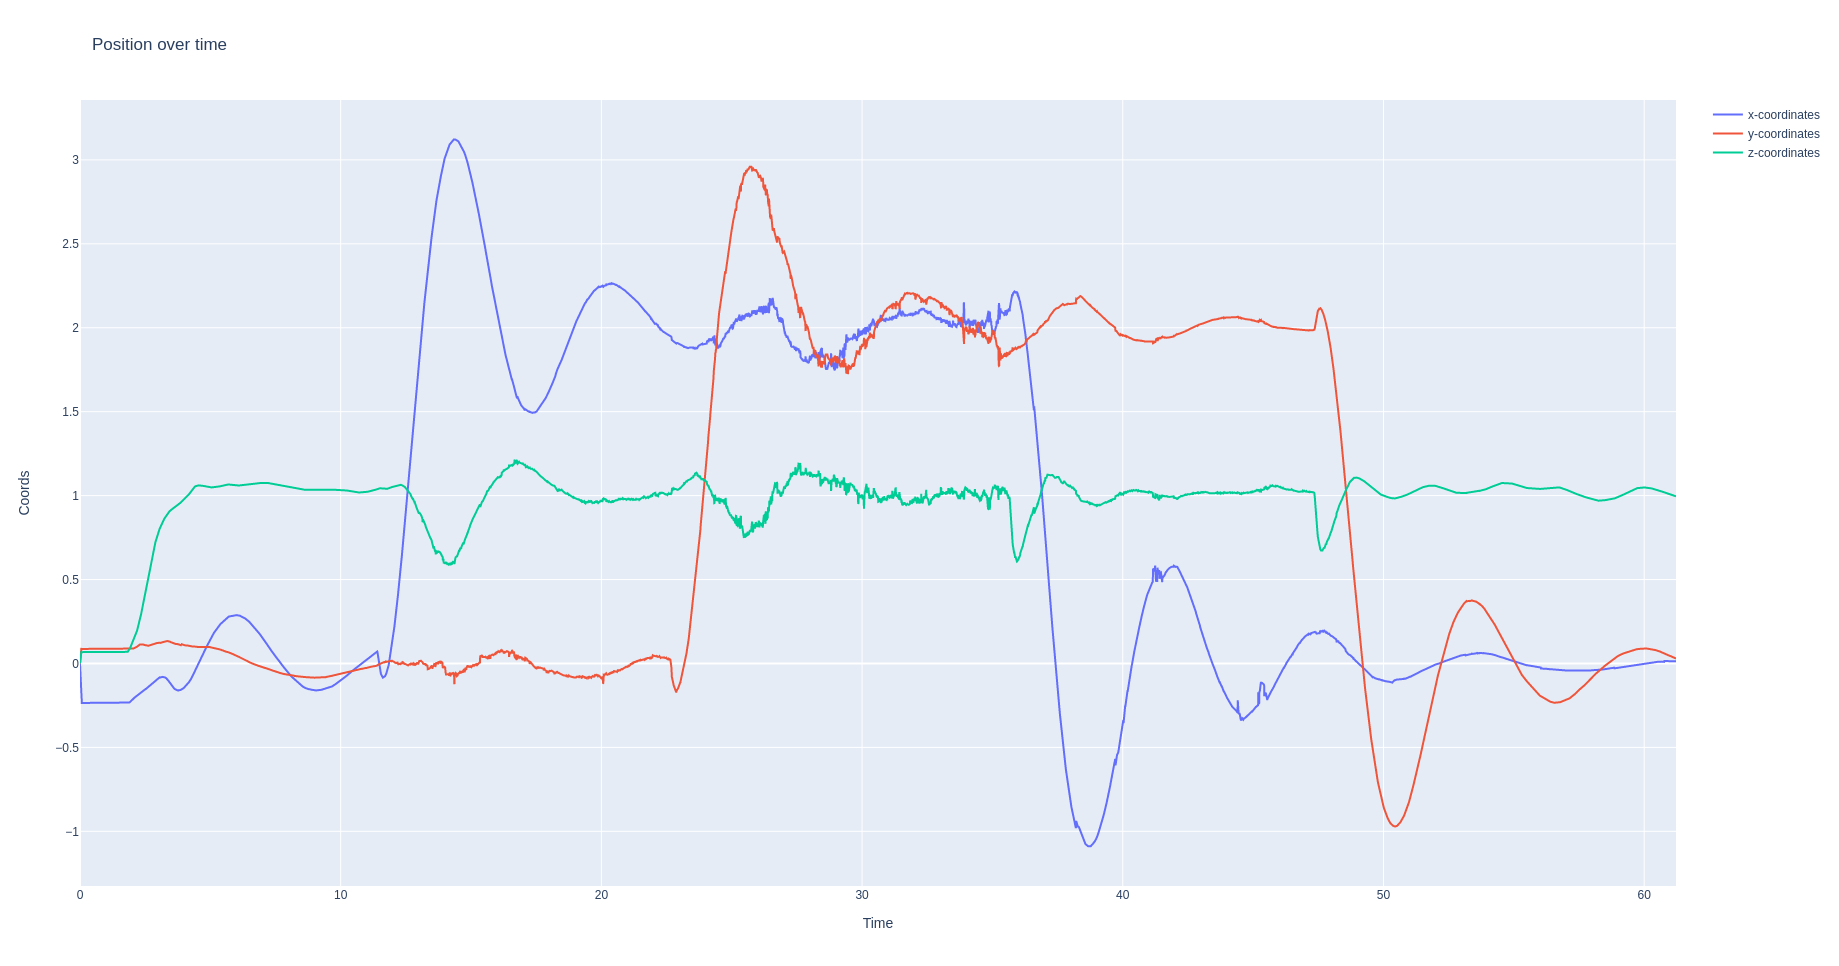
\includegraphics[width=1.0\linewidth]{images/task2_2_pos.png}
	\caption{x, y and z coordinates of the UAV. ( $K_p = 0.3$, $K_i = 0.01$, $K_d = 0.1$)}
	\label{fig:task2_2_pos}
\end{figure}

\begin{figure}[hbtp]
	\centering
	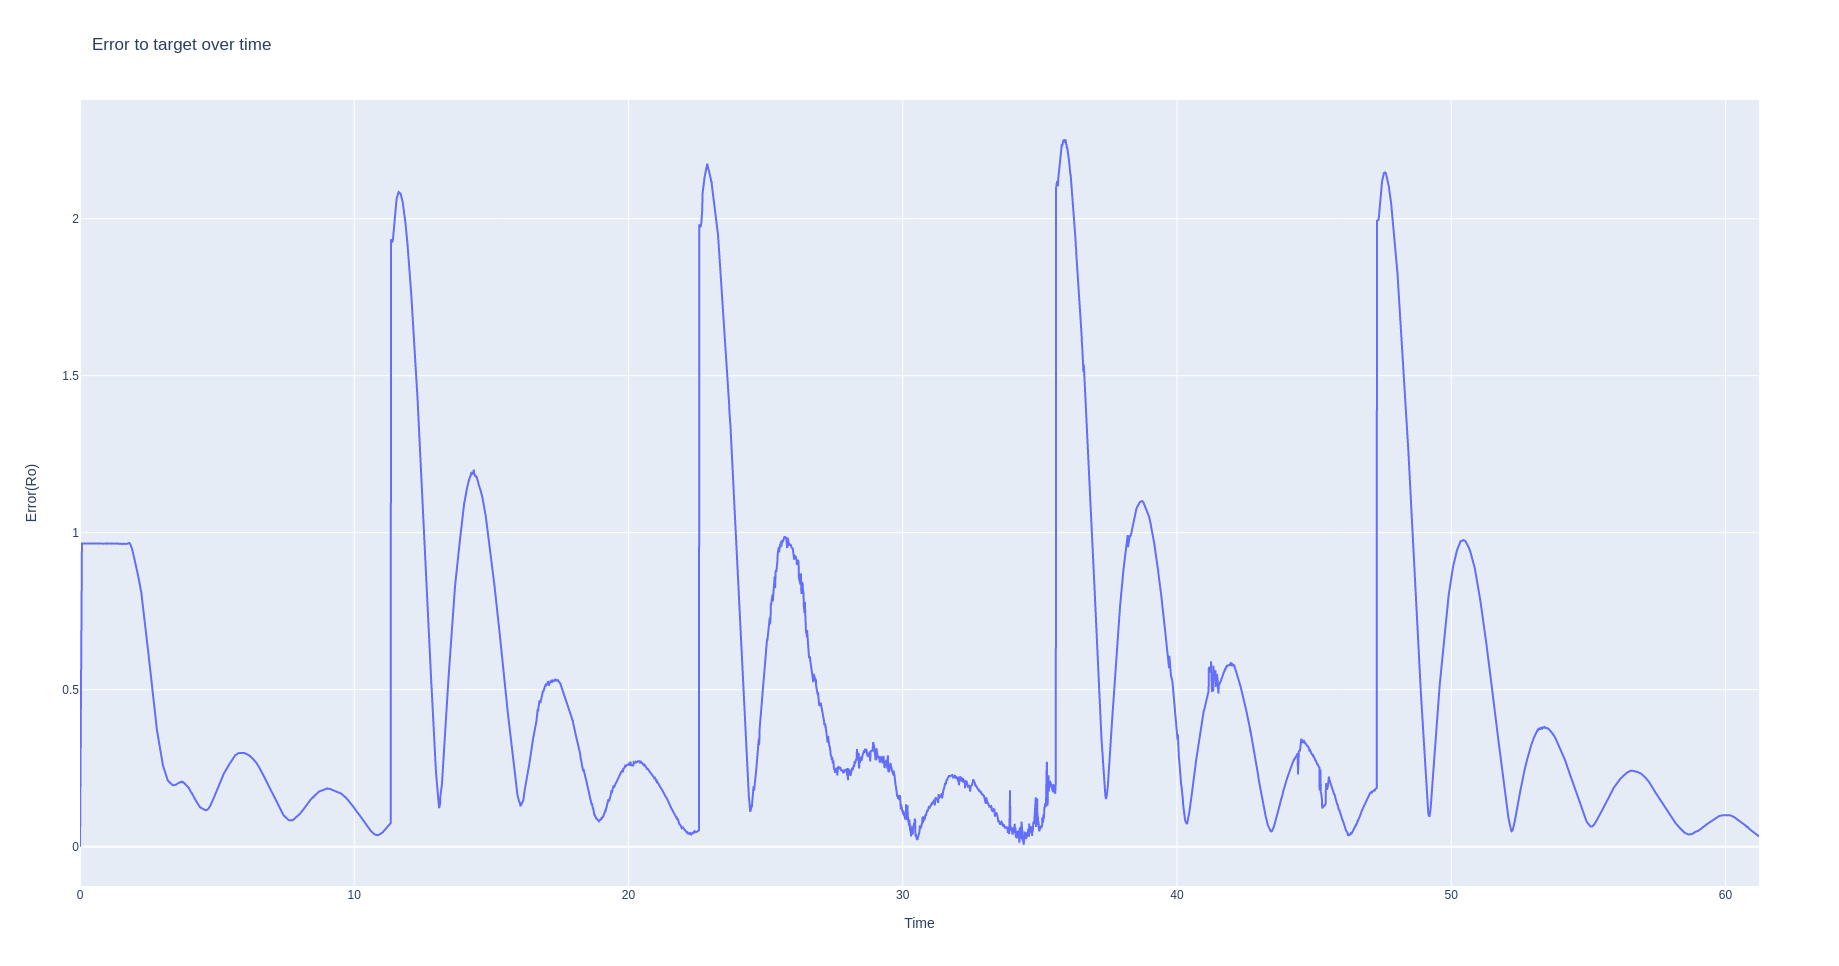
\includegraphics[width=1.0\linewidth]{images/task2_2_err.png}
	\caption{Error(distance) to way-points. ( $K_p = 0.3$, $K_i = 0.01$, $K_d = 0.1$)}
	\label{fig:task2_2_err}
\end{figure}

The result is very similar to when controller parameter $k_i$ was increased with an overshoot of around 50\%, but the UAV visits the four way-point twice as fast. This is because when $K_p$ is increased, the current error has a bigger influence on the controller output which makes the UAV tend to make a bigger overshoot and increasing the settling time. But compared to the integral part of the algorithm the proportional part becomes negative the moment the UAV overshoots its target, which doesn't make its settling time as bad. 
For the optimal PID-controller the same values from task 1 has been used, $K_p = 0.4$, $K_i = 0.02$, $K_d = 0.4$. 
The proportional and derivative has been increased 4 times compared to the base controller to increase the speed in terms of rise time and minimize the overshoot and settling time. The integral part has only been increased 2 times as the integral part is mostly used to eliminate steady-state error, which wasn't a problem in the base controller. The results of the optimal controller can be seen on \cref{fig:task2_6_pos} and \cref{fig:task2_6_err}. The optimal controller parameter values are: $K_p = 0.4$, $K_i = 0.02$, $K_d = 0.4$.

\begin{figure}[hbtp]
	\centering
	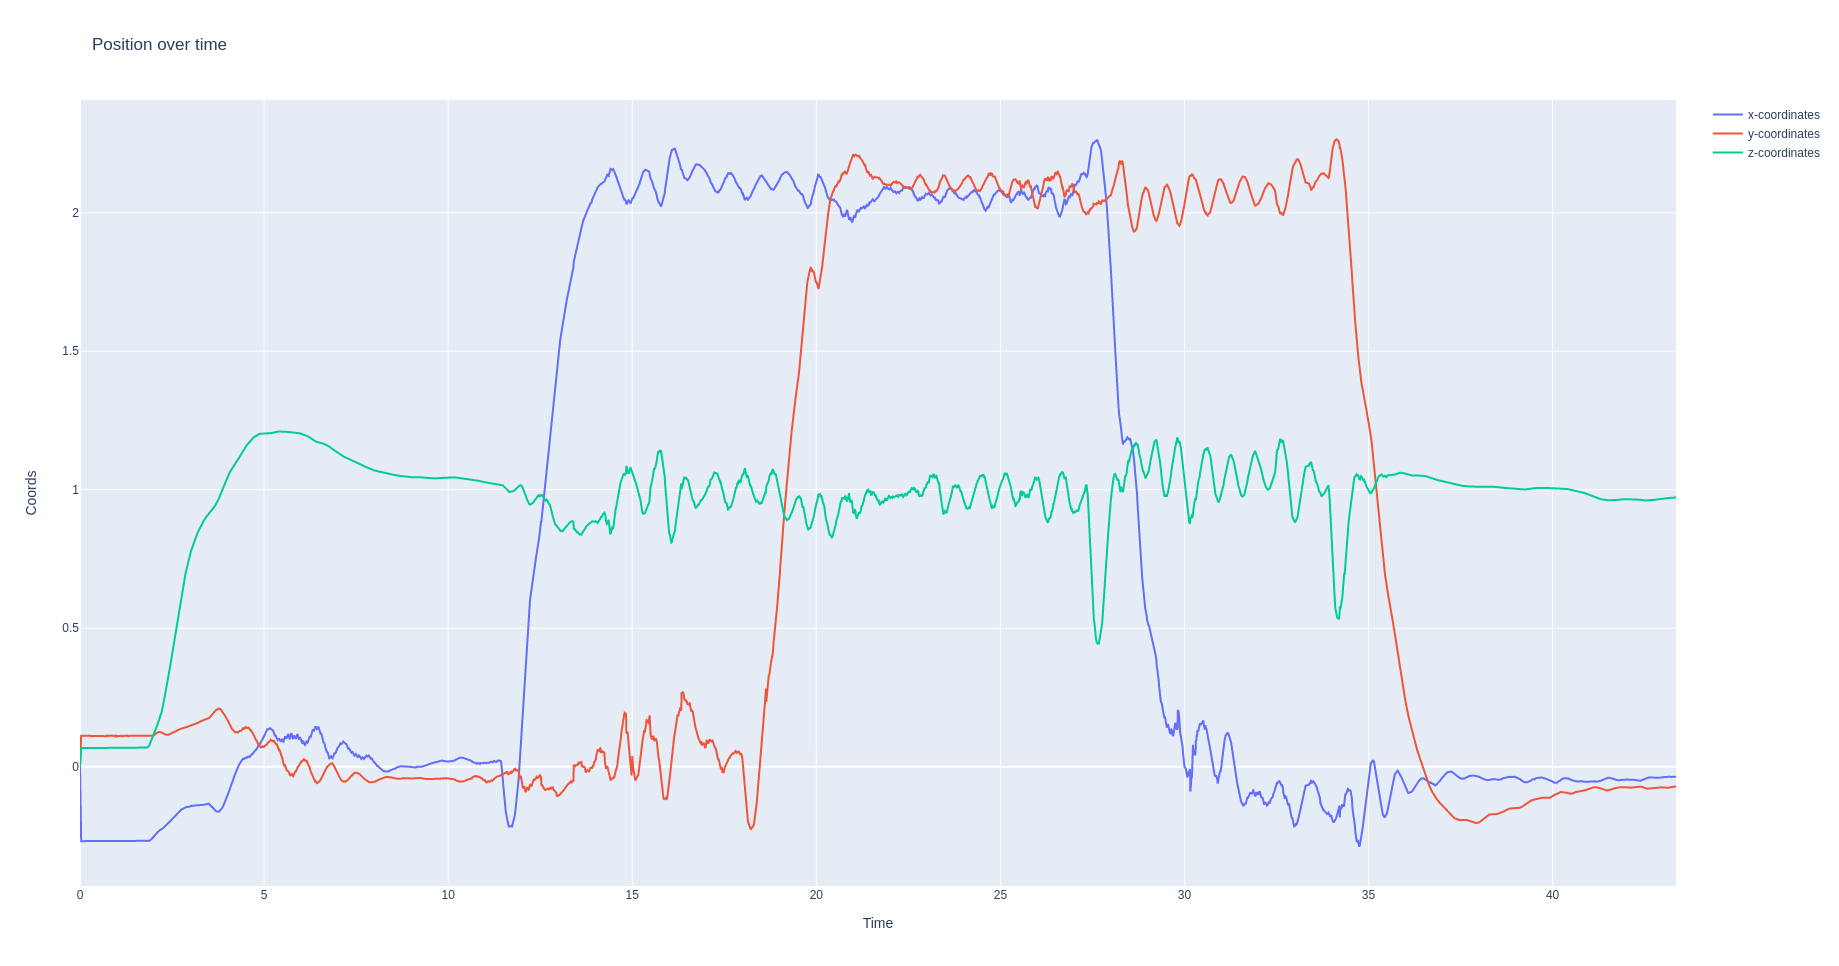
\includegraphics[width=1.0\linewidth]{images/task2_6_pos.png}
	\caption{x, y and z coordinates of the UAV. ( $K_p = 0.4$, $K_i = 0.02$, $K_d = 0.4$)}
	\label{fig:task2_6_pos}
\end{figure}

\begin{figure}[hbtp]
	\centering
	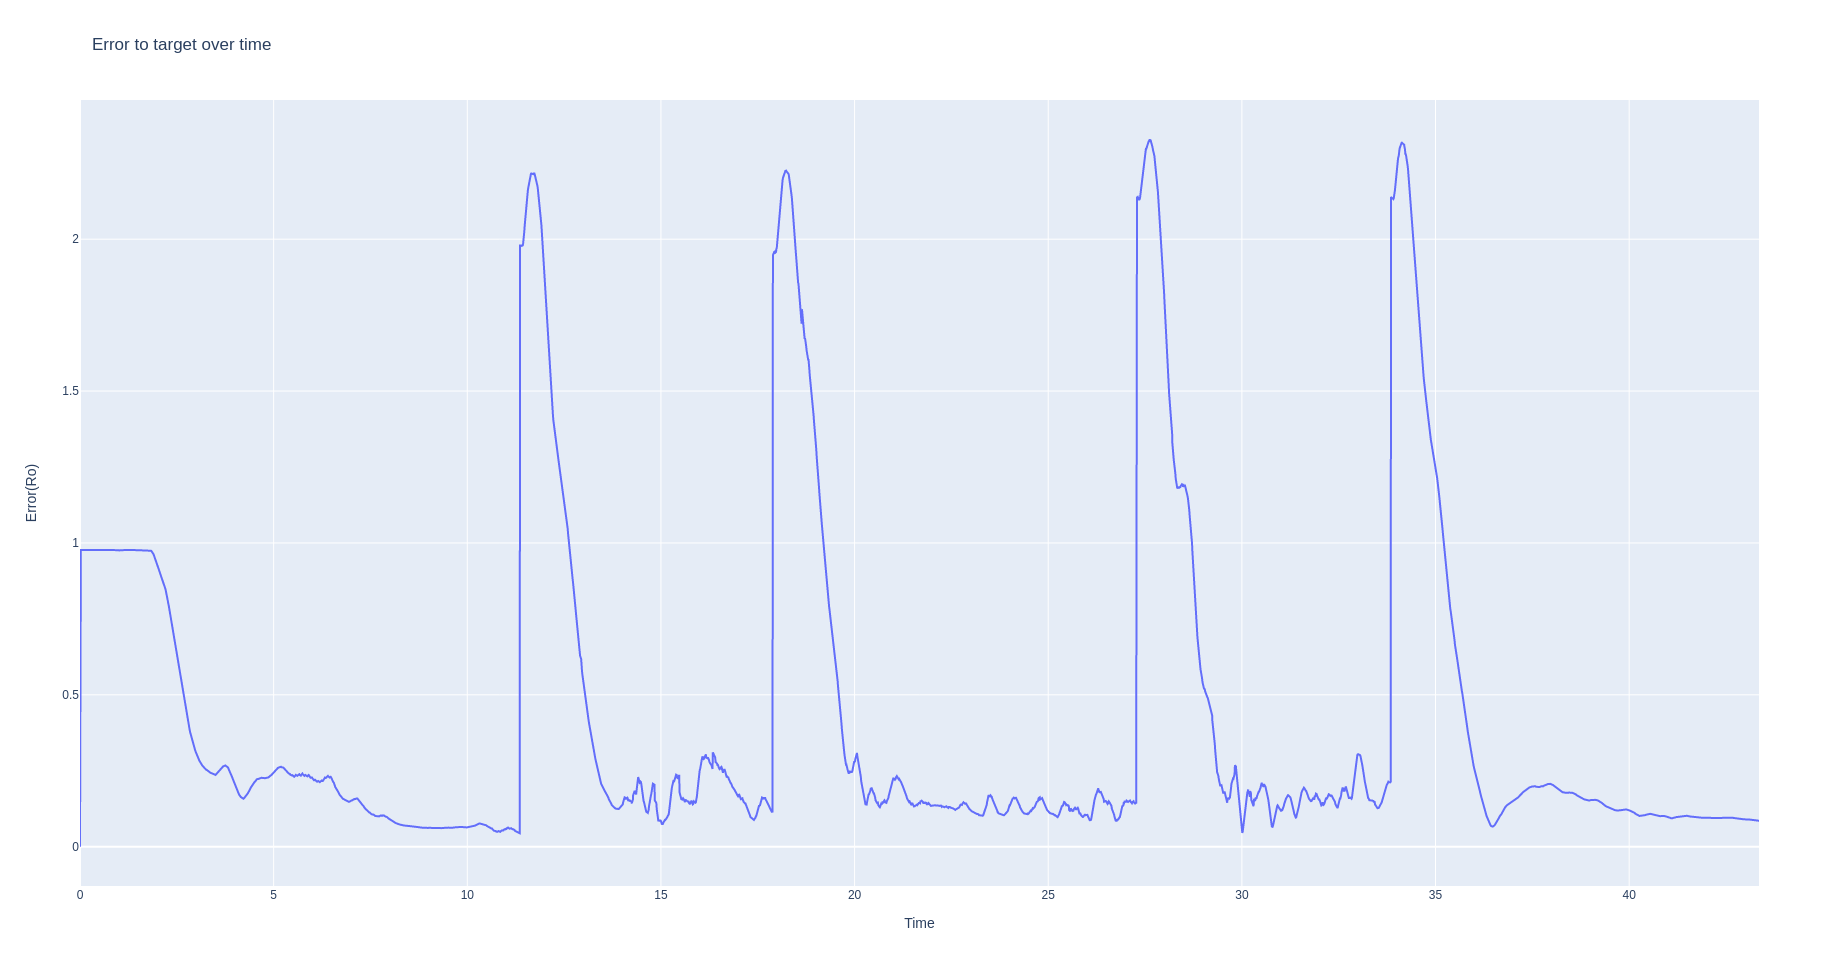
\includegraphics[width=1.0\linewidth]{images/task2_6_err.png}
	\caption{Error(distance) to way-points. ( $K_p = 0.4$, $K_i = 0.02$, $K_d = 0.4$)}
	\label{fig:task2_6_err}
\end{figure}

The results of the optimal controller show how the UAV visits the 4 way-points 20 seconds faster than the basic controller on \cref{fig:task2_1_pos} and \cref{fig:task2_1_err}, with almost no overshot. This is a very satisfying result showcasing how manual PID-controller tuning can improve the behaviour controller massively.

\section{Conclusion}
The objective of this final project were to design and implement a PID-controller, that would be able to control a Parrot Bebop 2 drone in the real lab environment. To accomplish this it have been necessary to transform linear velocity in inertial coordinates into the UAVs body frame. Another objective in this project have been to investigate the influence of the different controller parameters, both individually and combined and plot the results. 

This project are divided into two different tasks. The first task of the project involve the UAV hovering one meter above the ground at a specific point while being exposed to disturbances, which would make it possible to see the behaviour of the controller. The second task of the project involve the UAV flying in a square shape trajectory by visiting the way-points (2,0,1), (2,2,1), (0,2,1) and (0,0,1). The experiments of this project was carried out in real world setting at the AU Air lab located in Skejby. Both these tasks were carried out with different controller parameters, to investigate the influence of $K_p$, $K_i$ and $K_d$ individually and combined in a real world scenario. The PID-controller together with the transformation of linear velocity in Inertial coordinates into the UAVs body frames were successfully implemented.

The results showed that the theoretically influence of the controller parameter matched the physical results obtained at AU Air lab. The plots showed that an increase in $K_p$ resulted in lower rise time steady-state error but increase in overshoot and more unstable system. An increase in $K_i$ resulted in lower rise time and steady-state but an increase in overshoot of state-state error and more unstable system. Last an increase in $K_d$ resulted lower overshoot and settling time and better stability but an decrease in rise time. 


\begin{thebibliography}{00}

\bibitem{ros} http://wiki.ros.org/, date: 3/10/2020

\bibitem{Week3} Erdal Kaycan, ``Control Of Mobile Robots, week 3: Ground Robot models``, 16th of September 2020

\bibitem{book} RANDAL W. BEARD and TIMOTHY W. McLAIN, SMALL UNMANNED AIRCRAFT Theory and Practice, 2012

\bibitem{b2} CHRobotics, 2020, Understanding Euler Angles, http://www.chrobotics.com/library/understanding-euler-angles

\bibitem{b3} Control of Mobile Robots, Week 2 slides from lecture.

\end{thebibliography}
\vspace{12pt}

\end{document}
